\documentclass[12pt, titlepage]{article}
\usepackage[a4paper,margin=2.3cm]{geometry}
\usepackage{graphicx}
\usepackage{mathpazo}
\usepackage{tabularx}
\usepackage[table]{xcolor}  
\usepackage{xparse}
\definecolor{Gray}{gray}{0.85}
\usepackage{amssymb}
\usepackage{color, colortbl}
\usepackage{authblk}
\usepackage{jneurosci}	

\renewcommand{\baselinestretch}{1.3} 
\begin{document}
	\begin{titlepage}
		\begin{center}
			
			{\LARGE   A comparison of computational methods for detecting bursts in neuronal spike trains and their application to human stem-cell derived neuronal networks}
			\\ \bigskip {\large Abbrev title: Comparison of burst detectors for spike trains
				\bigskip \\  Ellese Cotterill$^{1^*}$, Paul Charlesworth$^2$, Christopher W. Thomas$^2$,  Ole Paulsen$^2$, Stephen J. Eglen$^1$
			}
		\end{center}
		\noindent$^1$Cambridge Computational Biology Institute, University of Cambridge, Wilberforce Road, Cambridge, CB3 0WA, UK
		\\$^2$Department of Physiology, Development and Neuroscience, Physiological Laboratory, Downing Street, Cambridge, CB2 3EG, UK
		\\$^*$Correspondence: Ellese Cotterill, University of Cambridge, Wilberforce Road, Cambridge,
		CB3 0WA, UK. E-mail: ec526@cam.ac.uk.
		\bigskip \\ \textbf{Conflict of Interest:} The authors declare no competing financial interests.
		\bigskip \\ \textbf{Acknowledgements:} Experimental data collection was supported by the BBSRC (PC, OP, grant number BB/H008608/1). CWT was supported by a bursary from the Bridgwater Summer Undergraduate Research programme. EC was supported by a Wellcome Trust PhD Studentship and NIHR Cambridge Biomedical Research Centre Studentship. We thank Tokdar et al., Pasquale et al., Ko et al., Gour\'{e}vitch et al. for code used in this study and Matthias Hennig for comments on the manuscript. 
		\bigskip \\ \textbf{Author Contributions:} EC, PC, OP and SJE designed research, EC and PC performed research, EC analysed data, EC, CWT and SJE contributed unpublished reagents/analytic tools, EC, PC and SJE wrote the paper.
	\end{titlepage}
	\subsection*{Abbreviations}
	\begin{tabular}{llll}
		\hline
		CMA & Cumulative moving average & MI & MaxInterval
		\\DIV &  Days \textit{in vitro} & PS &  Poisson surprise
		\\hiPSC & Human induced pluripotent stem cell \ \ \ &  RGC & Retinal ganglion cell
		\\HSMM &  Hidden semi-Markov model & RGS & Robust Gaussian surprise
		\\IRT & ISI rank threshold &	RS & Rank surprise
		\\ISI &  Inter-spike interval & WAP & Weeks after plating
		\\MEA & Microelectrode array & 
		\\ \hline
	\end{tabular}
	\section*{ABSTRACT}
	Accurate identification of bursting activity is an essential element in the characterisation of neuronal network activity. Despite this, no one technique for identifying bursts in spike trains has been widely adopted. Instead, a large number of methods have been developed for the analysis of bursting activity, often on an ad-hoc basis. Here, we provide an unbiased assessment of the effectiveness of eight of these methods at detecting bursts in a range of spike trains. We develop a list of features that an ideal burst detection technique should possess, and use synthetic data to assess each method in regards to these features. We further employ each of the methods to re-analyse microelectrode array (MEA) recordings from mouse retinal ganglion cells, and examine their coherence with bursts detected by a human observer. We show that a number of common burst detection techniques perform poorly at analysing spike trains with a variety of properties. We identify a small number of promising burst detection techniques, which are then applied to MEA recordings of networks of human induced pluripotent stem cell-derived neurons, and used to describe the ontogeny of bursting activity in these networks over several months of development. We conclude that there are a small number of burst detection methods that outperform others, however no current method can provide perfect burst detection results across a range of spike trains. We provide recommendations for the robust analysis of bursting activity in experimental recordings using current techniques.
	\section*{SIGNIFICANCE STATEMENT}
	Analysis of patterns of neuronal bursting is an important aspect in many studies of neuronal activity. A large variety of methods have been previously proposed for identifying bursts in neuronal spike trains, which take a range of different approaches. Here, we provide an unbiased quantitative assessment of eight existing burst detection methods, using both synthetic and experimental data. We reveal limitations in a number of commonly used burst detection techniques and provide recommendations for the best practice for accurate detection of bursts using a combination of existing techniques. 
	\section*{INTRODUCTION}
	The tendency of neurons to fire brief periods of spikes in quick succession, or bursts, has been observed extensively both \textit{in vitro} and \textit{in vivo} \cite{Weyand2001,Pasquale2010}. Bursting is believed to be associated with a variety of physiological processes, such as the formation of new synapses \cite{Maeda1995} and long term potentiation \cite{Lisman1997}. Using recordings of the electrical activity of neurons cultured on microelectrode arrays (MEAs), various aspects of \textit{in vitro} network activity, including bursting, can be readily examined. MEAs have thus been used to study changes in the spontaneous activity patterns exhibited by neuronal networks over development \cite{Wagenaar2006,Charlesworth2015}. Analysis of bursting activity has also been employed as an important tool in applications such as studying the impact of genetic or chemical manipulations on network activity \cite{Eisenman2015,Charlesworth2016}. 
	\\ \\ Despite the prevalence of bursting as a feature used to study neural network activity, the concept of a burst still lacks a definitive formal definition \cite{Cocatre-Zilgien1992} or single widespread technique used for detecting bursts. Instead, a variety of burst detection methods exist, many of which have been developed and verified by researchers on an ad hoc basis using specific data sets and singular experimental conditions. 
	\\\\One common approach to burst detection is to identify periods of bursting using simple thresholds, which impose limits on such values as the minimum firing rate or maximum allowed inter-spike interval (ISI) in a burst. These thresholds can either be fixed values  \cite{Cocatre-Zilgien1992,Chiappalone2005,Mukai2003},  or derived from properties of the spike trains, such as the mean ISI \cite{Chen2009}, firing rate \cite{Pimashkin2011} or some form of the distribution of ISIs or discharge density \cite{Selinger2007,Pasquale2010,Kaneoke1996,Bakkum2013,Kapucu2012}. Another type of burst detection techniques are the 'surprise-based' measures, which detect bursts as deviations from an assumed underlying firing rate distribution \cite{Legendy1985,Ko2012,Gourevitch2007}. There are also a variety of methods based on some combination of these ideas, or which take other approaches entirely \cite{Hennig2011,Tokdar2010,Turnbull2005,Tam2002,Xia2003,Wagenaar2005,Weihberger2013}.
	\\ \\ Most existing studies involving analysis of bursting activity in MEA recordings have been performed on experimental data from rodent nervous systems \cite{Charlesworth2015,Mazzoni2007}. In recent years, it has been demonstrated that networks of neurons derived from human stem cells can be grown successfully on MEAs, and exhibit spontaneous electrical activity, including bursting behaviour \cite{Illes2007,Heikkila2009}. %The suitability of these networks for applications such as neurotoxicity testing has also been demonstrated \cite{Yla-Outinen2010}. 
	There is thus a demand for the development of robust standardized analysis methods for identifying bursting in such networks, which often exhibit far more variable and less well defined bursting behaviour than more commonly studied rodent neuronal networks \cite{Kapucu2012}.
	\\ \\ Here, we have reviewed a number of existing burst analysis methods and evaluated their effectiveness at detecting bursts, particularly in spike trains with properties resembling those of human stem cell-derived neuronal networks. Each burst detection technique was used to analyse bursts in both synthetic spike trains simulated to exhibit common properties of human network recordings, as well as \textit{in vitro} MEA recordings from mouse retinal ganglion cells (RGCs). This allowed for an unbiased quantitative assessment of the performance of each method in a variety of contexts. Based on these results, we offer suggestions to researchers regarding the best approaches for comprehensive burst analysis. The highest performing methods in our study were also employed describe the ontogeny of bursting activity in neuronal networks derived from human induced pluripotent stem cells (hiPSCs) over several months of development. 
	\section*{MATERIALS AND METHODS}
	\subsection*{Burst analysis methods}
	Eight burst detectors that we believed to be representative of the major approaches to burst detection, and that have sufficient general applicability to allow for their use on a variety of spike trains, were chosen for analysis. Other methods were excluded from the analysis for a variety of reasons, including that they do not explicitly identify the location of bursts in a spike train \cite{VanElburg2004}, or we believe that they were superseded by other methods that were adapted from them \cite{Selinger2007,Chiappalone2005}. 
	\\ \\ A brief description of each of these methods applied to a single spike train is given below, and we refer the reader to the original sources for more detailed descriptions. Where possible, we also reused existing code to implement each method. To minimise the impact of our implementation on the evaluation of each burst detection technique, in general the parameters used in each method were the standard parameters suggested by the authors, and are shown in Table \ref{param_vals}.  For all methods, the minimum number of spikes in a burst was set to three. 
	\\ \\ \textit{LogISI method \cite{Pasquale2010}} 
	\\Bursts are detected using the histogram of the log adjusted inter-spike intervals (ISIs) on a spike train. The peaks of this histogram are found, and the largest peak corresponding to an ISI of $100\,$ms or less is set as the intra-burst peak. In the absence of such a peak, no bursts are found. The minimum values between the intra-burst peak and all subsequent peaks are found, and a void parameter, which represents how well the peaks are separated, is calculated for each minima. The ISI value corresponding to the first minimum at which the void parameter exceeds a threshold value of 0.7 is set as the cutoff value for burst detection, $maxISI$.  Bursts are then detected as any series of three or more spikes separated by ISIs smaller than $maxISI$. If no cutoff is found, or if $maxISI>100\,$ms, bursts are found using a $100\,$ms cutoff, and then extended to include any spikes within $maxISI$ of the edges of each burst.
	\\ \\ \textit{Cumulative Moving Average (CMA) method \cite{Kapucu2012}} 
	\\The cumulative moving average (CMA) of the histogram of ISIs is found. The skewness of this CMA distribution is used to determine the values of two parameters, $\alpha_1$ and $\alpha_2$,  according to the scale given in \cite{Kapucu2012} and shown in Table \ref{param_vals}. The ISI value of the histogram bin at which the CMA is closest in value to $\alpha_1 \cdot CMA_{MAX}$, is set as $maxISI$, where $CMA_{MAX}$ is the peak of the CMA distribution. Again, bursts are defined as sequences of more than two spikes separated by ISIs less than $maxISI$.
	\\ \\ The authors of this method also suggest expanding these bursts to include burst related spikes, which are found using a cutoff set at the histogram bin at which the CMA is closest to $\alpha_2 \cdot CMA_{MAX}$. Any spikes within this cutoff distance from the beginning or end of the original bursts are classified as burst related spikes. However, for our purposes, we only examined the original burst cores detected from this method, and did not include any burst related spikes.
	\\ \\ \textit{ISI rank threshold (IRT) method \cite{Hennig2011}}
	\\The rank, $R(t)$, of each ISI relative to the largest ISI on the spike train is calculated. A rank cutoff, $\theta_R$, is chosen, and a spike count cutoff, $\theta_C$, is calculated from the distribution of spike counts over one second intervals of the spike train. A burst begins at a time $t$ if the spike count over the following second exceeds $\theta_C$, and its subsequent ISI satisfies $R(t)<\theta_R$. The burst continues until the spike count over the proceeding one second interval falls below $\frac{\theta_C}{2}$.
	\\ \\ \textit{Poisson Surprise (PS) method \cite{Legendy1985}}
	\\The baseline firing rate on a spike train is assumed to follow a Poisson process with rate, $\lambda$, equal to the mean firing rate over the entire train. The Poisson surprise statistic for an interval of length $T$ containing $N$ spikes is defined as 
	\[S = -\log(p)\] 
	where $p$ is the probability of $N$ or more spikes randomly occurring in an interval of length $T$ in the underlying Poisson process. Bursts are chosen so as to maximise the Poisson surprise statistic over the entire spike train using a surprise maximisation algorithm outlined in \cite{Legendy1985}, and any bursts with a Poisson surprise value below a threshold significance level are discarded. In our implementation, the cutoff significance level was reduced from the value of ten, used in \cite{Legendy1985}, to a value of $-\log(0.01)\approx 4.6$, to bring it in line with the other surprise methods.
	\\ \\ \textit{Rank Surprise (RS) method \cite{Gourevitch2007}}
	\\The length of ISIs on the spike train are ranked,  with the smallest ISI given a rank of 1. For each possible bursting interval, the rank of all ISIs on the interval are summed, and the probability, $p$, of a value of equal of lesser value  being drawn randomly from a discrete uniform sum distribution is calculated. Bursts are chosen so as to maximise the rank surprise statistic, defined as $RS=-\log(p)$, across the entire spike train, and any bursts with a rank surprise statistic below a pre-defined significance threshold are discarded\nocite{Gourevitch2007}. 
	\\ \\ \textit{Robust Gaussian Surprise (RGS) method \cite{Ko2012}}
	\\Bursts are regarded as outliers from a ``central distribution'' of ISIs, which is estimated by normalising the distribution of $\log(ISIs)$ on the spike train. ISIs are considered to be potentially within bursts if they lie below -2.58 times the median absolute deviation of this distribution. For each potential burst, the Robust Gaussian Burst Surprise value, $GS_B=-\log(p)$, is calculated, where $p$ is the probability that the sum of the normalized $\log(ISIs)$ in the interval is less than or equal to the sum of an equivalent number of i.i.d. Gaussian random variables with mean and standard deviation equal to those of the central distribution. These initial bursts are then extended to include surrounding spikes until the maximal surprise value is found. Finally, any bursts with a surprise value below a pre-defined significance threshold are discarded.
	\\ \\ \textit{Hidden Semi-Markov Model (HSMM) method \cite{Tokdar2010}}
	\\Neurons are assumed to stochastically alternate between a ``non-bursting'' and ``bursting'' state, labelled states 0 and 1 respectively. Spiking activity is modelled using a hidden semi-Markov model, with transition times between the two states modelled as two Gamma distributions,  $f_0^{ITI}$ and $f_1^{ITI}$.  Within each of the two states, the distribution of ISIs are modelled using additional Gamma distributions, $f_0^{ISI}$ and $f_1^{ISI}$. The parameters of these four distributions are learned from the data. Under these assumptions, the posterior probability that the neuron is in a bursting state at any given time is calculated using a Markov chain Monte Carlo (MCMC) method, and any periods in which this probability exceeds a threshold value are classified as bursts.
	\\ \\ \textit{MaxInterval (MI) method  \cite{NEmanual}}
	\\Any series of consecutive spikes fulfilling five user-inputted threshold parameters are classified as bursts. For our purposes, the values of the parameters were those specified in the NeuroExplorer Manual, and shown in Table \ref{param_vals}.
	\subsection*{Analysis of synthetic data}
	The performance of each method was evaluated against a list of desirable properties, shown in Table \ref{des_prop}. For properties D1-D3, performance was based on the details of the method's implementation, while for the remaining properties, testing on simulated data was performed. Simulated data was used for this purpose because it allowed us to generate spike trains with specific properties of interest, and provides the `ground truth' of bursting behaviour to compare with the results of each method. Simulated spike trains were produced using the models outlined below, with the parameter values specified in Table \ref{sim_params}.
	\\\\ 	\textit{Poisson and Gamma distributions}
	\\Two types of non-bursting spike trains were simulated, one with Poisson distributed ISIs, and the other with Gamma distributed ISIs. The smallest 10th percentile of ISIs were removed from each spike train, to eliminate any burst-like behaviour arising randomly in the simulated data.
	\\ \\  \textit{Inhomogeneous Poisson distribution}
	\\ Spike trains with non-stationary firing rates and no bursts were simulated using a Poisson process with non-homogeneous intensity, $\lambda(t)$. To eliminate any possible bursting behaviour, the smallest 10th percentile of ISIs were removed from each simulated spike train.
	\\ \\  \textit{Poisson Bursting}
	\\ Bursting spike trains were simulated using the Poisson bursting model. The location of the centre of each burst on a spike train was modelled using a Poisson process with a fixed rate, $\lambda$. The number of spikes in each of the bursts was drawn from a Poisson distribution with mean $n$. The position of the spikes relative to the burst centre were drawn from a uniform distribution with range $r$ and mean 0. Where two bursts overlapped, only the first was kept. 
	\\ \\ To simulate noise in bursting spike trains, noise spikes were modelled with Gamma distributed ISIs with the smallest 10th percentile of ISIs removed. This was overlaid on the Poisson bursting spike train and any noise spikes within $0.5 \,$s of the limits of each burst were removed, to prevent any overlap between burst and noise spikes.
	\\ \\ For each desirable property, one hundred spike trains of duration 300$\,$s were simulated and analysed using each of the burst detection techniques detailed above. Examples of the simulated spike trains used to assess each desirable property are shown in Figure \ref{sim_egs}. A comparison of the `ground truth' bursting behaviour and the results from each method was then performed. 
	\subsection*{Analysis of RGC data}
	MEA recordings of mouse RGC from \cite{Demas2003} were re-analysed using the burst detection methods in our study. Four hour-long recordings of  control mice retina at postnatal days 9, 11, 13 and 15 were chosen for re-analysis. For spike trains from five randomly chosen electrodes from each recording, the `ground truth' bursts were annotated by visual inspection by one of the authors (EC). Examples of annotated bursts for spike trains at each age are shown in Figure \ref{RGC_eg}. For each method in our study, bursts were detected on the annotated spike trains using a variety of input parameters, and the sensitivity and specificity of each method examined.
	\\ \\The parameter that was varied in the HSMM and surprise methods was the probability cutoff, while for the ISI rank threshold method, the spike count cutoff, $\theta_C$, was altered. For the logISI method, the limit on the maximum allowed ISI cutoff value was varied from its initial value of 100$\,$ms. For the MI method, most parameter values shown in Table \ref{param_vals} were maintained, excluding the maximum beginning and end ISIs, which were varied so that the maximum end ISI was always 0.130$\,$s greater than the maximum beginning ISI. Finally, for the CMA method, for which there were no obvious parameters to vary, only a single value for sensitivity and specificity was found.
	\\ \\ ROC curves were created that plotted 1-specificity versus sensitivity for various parameter values. Sensitivity was defined as the number of spikes correctly detected as being within bursts, as a fraction of the total number of spikes in the annotated `ground truth' bursts. The value of 1-specificity, or the false positive rate, was the number of spikes that were falsely detected as being within bursts, as a fraction of the total number of spikes that were not a part of the `ground truth' bursts.
	\subsection*{Experimental details for hiPSC derived neural network recordings}
	To complete, with Paul's input.
	\section*{RESULTS}
	\subsection*{Desirable properties for a burst detector}
	To evaluate the performance of each burst detector, the methods were assessed against ten desirable properties, listed in Table \ref{des_prop}. The optimal burst detector would ideally possess all of these desirable properties. For binary properties, D1-D4, each method was judged to either possess the property or not, while for properties D5-D10, the performance of each method was ranked against the other methods, based on its median performance in analysing one hundred synthetic spike trains. 
	\\ \\ The first desirable property of a burst detector was that it was deterministic (D1), as this ensures reproducibility and removes the need to find a `consensus' set of bursts across repeated trials. The only non-deterministic method was the HSMM method, due to its use of MCMC methods. The bursts detected this method varied considerably between trials. For example, with repeated analysis of a simulated $300\,$s Poisson bursting spike train with burst frequency of 0.2$\,$Hz by the HSMM method, the number of bursts detected on the spike train varied from 2 to 56 bursts over one hundred trials. 
	\\ \\ Another desirable property for the burst detection methods was that they did not assume that ISIs on a spike train follow a specific statistical distribution (D2). There is no consensus on which type of statistical distribution best represents underlying spike train activity%(ref?)
	, and any assumption that this activity follows a fixed statistical distribution restricts the applicability of a method to a narrow range of spike trains. Most methods do not assume a fixed statistical distribution for the underlying spike train, excluding the PS, RGS and HSMM methods, which assume that ISIs can be modelled using a Poisson process, Gaussian distribution and Gamma distributions respectively. However, these methods remain somewhat robust to departures from these assumptions, as `surprising' sequences of spikes as measured by one distribution, will generally also correspond to high surprise values from other distributions commonly used to model spike trains \cite{Legendy1985}. 
	\\ \\ A common issue that arises when applying burst detection techniques to large sets of spike trains that have high variability in their statistical properties, such as those obtained from MEA recordings of human neuronal networks, is how to accurately choose the parameters for burst detection. This is further confounded when burst detection methods are applied to MEA recordings spanning a large range of developmental ages, or differing experimental conditions. Thus, ideally, a burst detection method should have a small number of parameters (D3), to minimise the impact of how parameter values effect the resultant detected bursts. Most methods in our study only required one or two input parameters. The MI method, on the other hand, required five parameters to be carefully specified to implement burst detection. The HSMM also requires a large number (N=27) of parameters to correctly fit the hidden semi-Markov model to the data, however many of these are initial values that are later optimised by the algorithm, and can be left set to the values suggested by the original authors with little impact on the effectiveness of the method. 
	\\ \\ With the increasing prevalence of high density MEAs that contain up to several thousand electrodes \cite{Maccione2014}, as well as the use of MEAs for high-throughput toxicology screening \cite{Breier2008}, the computational complexity of each of the methods must also be considered. To assess computational time (D4), each method was used to analyse one hundred five minute simulated spike trains with average firing rate of 1$\,$Hz. The majority of methods required on average only a fraction of a second to analyse each spike train using a standard personal computer. The exception to this was the HSMM method, which had an average computational time more than 20 times greater than any of the other methods. Extrapolating from this, using the HSMM method to analyse a recording from one high-resolution array of 4096 electrodes may require several hours, compared to a few seconds or minutes using the other methods.
	\\ \\ A common feature seen in recordings of human neuronal networks is the presence of electrodes that record sparse or no bursting behaviour, with either relatively stationary or quite variable firing rates over the course of the recording. An ideal burst detection method would find no or very little bursting activity in these spike trains. Most burst detectors performed reasonably well at detecting a low amount of bursting activity in spike trains simulated to exhibit an absence of bursting behaviour (D5). The major exception to this was the HSMM method, which had a tendency to significantly overestimate bursting behaviour in these trains (Figure \ref{sim_results1}A).  
	\\ \\ When the property of a non-stationary firing rate was added to the non-bursting trains (D6), the number of erroneous bursts detected by the majority of methods increased (Figure \ref{sim_results1}B). The CMA method, in particular, showed a significant increase in the amount of bursting activity detected in non-stationary spike trains, compared to those with a static firing rate. This can be attributed to the fact that the CMA method tends to detect periods of 'unusual' activity as bursts, and thus showed a tendency to detect bursts in the regions of relatively high firing rate in these spike trains.
	\\ \\ An ideal burst detector should also be able to detect bursts accurately in spike trains that contain only bursting behaviour, especially those in which the bursts are regular and well separated (D7). Most methods possessed this property, and could identify over 90\% of the spikes as bursting in simulated spike trains with regular bursting behaviour (Figure \ref{sim_results1}C). The exceptions to this were the RS, IRT and RGS methods, which consistently detected less than half of the bursts in the synthetic data.
	\\ \\ We also analysed the performance of each method on simulated spike trains with less standard bursting behaviour. This included  spike trains containing bursts with long durations and relatively low within-burst firing rates (D8). For these spike trains, only the PS and HSMM methods gave reasonably accurate results for both the proportion of spikes in bursts and the number of bursts in the spike train. The MI and CMA methods both correctly allocated a large proportion of the spikes as being within bursts, but had a tendency to separate the long bursts into shorter, more frequent bursts, while the remaining methods greatly underestimated the prevalence of bursting behaviour in the simulated data (Figure \ref{sim_results2}A,B).
	\\ \\ Another type of non-standard bursting behaviour seen in human network recordings is the presence of short, poorly separated bursts occurring at a high frequency. When used to analyse spike trains with very frequent bursting behaviour (D9), the MI, logISI and HSMM methods were able to correctly identify the majority of spikes as being within bursts, but had a tendency to combine the short bursts into a smaller number of longer bursts. The CMA method most accurately detected the large number of bursts on these high frequency spike trains, but had a tendency to underestimate the proportion of spikes in bursts. The RS, IRT and RGS methods, on the other hand, were only able to identify a low proportion of bursting spikes and low number of bursts in these spike trains (Figure \ref{sim_results2}C,D).
	\\ \\ Finally, an ideal burst detector should be able to correctly differentiate between bursting and non-bursting periods in spike trains in which some spiking activity occurs outside of bursts (D10). By comparing each method's output to the ground truth bursting behaviour in simulated spike trains containing both bursts and noise, we were able to examine the fraction of spikes that were correctly identified as being within bursts, as well as the fraction of between-burst, or noise spikes, that were erroneously detected as being within bursts by each method.
	The PS, MI, CMA, logISI and HSMM methods had reasonably high true positive rates for identifying bursting spikes, however, of these, the logISI and HSMM methods tended to allocate a higher proportion of noise spikes as being within bursts (Figure \ref{sim_results2}E,F). The RS, IRT and RGS methods exhibited very low false positive rates, but this came at the expense of quite low true positive rates, giving them low overall recall.
	\\ \\ The performance of each of the methods across all desirable properties is summarised in Tables \ref{des_results1} and \ref{des_results2}. The ranking in Table \ref{des_results2} was based on the median and range of the boxplots in Figures \ref{sim_results1} and \ref{sim_results2}, with methods with similar results given equal rankings.
	% Based on the properties D1-D4 in Table 1, the HSMM method has the worst performance in terms of its computational complexity and underlying assumptions. For the desirable properties requiring testing on simulated data in Table 2, however, it is the RS, IRT and RGS methods that significantly underperform the other methods. 
	\subsection*{Preliminary analysis of mouse RCG data}
	MEA recordings from \citetext{Demas2003}, a study which examined the changes in spontaneous retinal activity in both normal and dark-reared mice over development, were re-analysed using the burst detection methods in our study. The sensitivity and specificity of each method at a range of parameter values was found according to the definitions outlined in the methods, and averaged across the five annotated spike trains from each recording, to create the ROC curves for each age shown in Figure \ref{ROC}. 
	Because of innate restrictions on how bursts are defined by each method, for example that bursts must contain a minimum of three spikes, many methods did not allocate either no spikes or 100\% of spikes as being within bursts for any choice of parameter values, and thus the ROC curves do not span the entire range of sensitivity and specificity values. The methods were thus assessed by their minimum distance from the point of ‘perfect’ classification at (0,1), rather than the area under the ROC curve.
	\\ \\The MI method exhibited strong performance across all ages, and was able to reach very high levels of sensitivity and specificity for a specific choice of parameter values at each age. The logISI, PS and CMA methods also had promising performance across most ages, however at P15 these methods exhibited consistently higher false positive rates (Figure \ref{ROC}D). The results from the RGS method did not vary significantly as its parameter value was changed, and it was unable to reach high levels of sensitivity for any choice of parameter values. The sensitivity and specificity of the RS and IRT methods, on the other hand, spanned a range of values, however these methods were unable to reach the levels of sensitivity of the other methods. The HSMM method reached high sensitivity levels, but only at the cost of low specificity, and generally performed poorly across all ages.
	\subsection*{Evaluation of the methods} 
	Based on the assessment of the methods against the desirable properties, the RGS, RS and IRT methods underperformed compared to other methods. This was reinforced through their performance when compared to human detection of bursts on mouse RGC data, where they were not able to reach the levels of sensitivity of the other methods in our study. These three methods were thus eliminated from any further analysis. The HSMM method had average performance on simulated data (D5-D10), however the complexity of the method's implementation meant that it was the lowest performing method on properties D1-D4. The high false positive rate of the method across all ages when analysing experimental data cemented our decision to remove this method from further examination. 
	\subsection*{Further analysis of mouse RGC data}
	The remaining four methods, namely the PS, MI, CMA and logISI methods, were used to analyse the complete set of spike trains from each of the four RGC recordings. In this case, the parameters used for this analysis were based on those that resulted in the best performance in the ROC curves above, as measured by the distance of the curve from the point of perfect classification in the top-left corner. In the original study of this data, rather than explicitly identifying spikes as being either within or between bursts, the authors gave a qualitative description of bursting activity based on visual analysis of the spike train, and used the autocorrelation of each spike train to determine the average burst duration on each recording. By explicitly identifying bursts using our four burst detectors, we were able to provide a more detailed description of the bursting behaviour and compare this with the authors' original results.
	\\ \\ The burst detectors were generally in agreement about the proportion of spikes in bursts across all ages, and showed an increase in the fraction of spikes occuring within burst between P9 and P15 (Figure \ref{RGC_results}). This is in agreement with the analysis of the original authors, who found that only very few spikes occurred outside of bursts at early ages, while by P15, many cells were active outside of bursts \cite{Demas2003}.
	\\ \\In terms of burst duration, all four methods showed very similar results over P9 to P13, which resemble the values found by the autocorrelogram method. However, at P15 there is a significant deviation between the results of the PS method and the other methods. The MI, CMA and logISI methods followed the trend of decreasing burst duration with age found in the original analysis, while the PS method detected a significant increase in burst duration at P15. This can be attributed to the fact that at P15, many spike trains exhibited regular `bursting episodes', periods of high activity generally spanning 10-20$\,$s that consisted of a series of shorter bursts. The PS method had a tendency to classify these bursting episodes as one long burst, while the other methods generally broke up these periods into several shorter bursts, as shown in the example spike train in Figure \ref{RGC_results}. 
	\subsection*{Analysis of hiPSC derived neuronal network recordings}
	Seventy-three recordings from networks of neurons derived from human induced pluripotent stem cells taken at regular intervals from two to fifteen weeks after plating were analysed using the four best burst detection methods. The MI, PS and logISI parameters used for this analysis were chosen by inspection as those that most accurately detected bursts on five randomly chosen spike trains with mean firing rate close to 1$\,$Hz, which is the minimum firing rate at which regular bursting behaviour tends to arise.  For the CMA method, the scale for $\alpha_1$ values in \citetext{Kapucu2012} were used, and the authors suggestions for post-hoc screening were employed, with any spike trains that were found to have average burst duration greater than 5 seconds or an average number of spikes per burst above 50, declared as non-bursting.  The resultant parameters for each method are shown in Table \ref{param_vals_hum}.
	\\ \\ Although there were some differences in the absolute level of bursting activity detected by the different analysis methods, the results from most methods suggested a general trend of `ramping up' of bursting, in terms of burst rate and percentage of spikes in bursts, with increasing developmental age (Figure \ref{hiPSN_results}). In general, however, the prevalence of bursting activity in these human network recordings tended to be significantly lower than that commonly seen in recordings of rat and mouse hippocampal or cortical networks \cite{Charlesworth2015,Chiappalone2005}.
	% %Could be a result of plating density - wagenaar?
	Also, unlike some previous studies of rodent neuronal networks \cite{Charlesworth2015,Demas2003}, there was no obvious relationship between burst duration and culture age, with bursts remaining short over the entire developmental period. Similarly, the degree of regularity of the bursting activity, captured by the CV of IBI, did not appear to change significantly with increasing developmental age.
	\\ \\ To gather insight on how bursts were being detected in these recordings, visual inspection of a subset of the spike trains was performed.  Figure \ref{hiPSN_examples} shows a number of example spike trains at 4, 8 and 12 weeks after plating (WAP), with the bursts detected by each method displayed. In a number of these examples, the CMA method failed to detect numerous periods that a human observer would generally classify as bursting (Figure \ref{hiPSN_examples}C, E). This may account for the lower burst rates and proportion of spikes in bursts found by this method, compared to the other methods (Figure \ref{hiPSN_results}B, C). Additionally, the PS method exhibited a tendency to combine bursts that other methods detected as separate bursts, and extend bursts to incorporate additional spikes that visual inspection would suggest should not be included in bursts. This may explain the longer burst durations found by this method (Figure \ref{hiPSN_results}A). Although no method agrees perfectly with how we would assign bursts in these spike trains by visual inspection, out of the four methods examined here, on average the MI method corresponds most closely to our visually detected bursts. 
	\section*{DISCUSSION}
	Despite the important role of accurate burst detection in analysing neuronal network activity in a variety of contexts and experimental conditions, a consistently widely used method for burst analysis is yet to be adopted. By examining the performance of eight existing burst detection techniques at analysing both synthetic and experimental data, we found that a number of burst detectors perform poorly at identifying bursts in spike trains with a variety of properties. We identified a small number of methods that outperformed compared to other existing methods, and used these to analyse bursting activity in recordings of hiPSC-derived neuronal networks over several months of development.
	\\ \\We have shown that a number of burst detectors that were developed based on recordings from single experimental conditions do not necessarily generalise to use on other types of spike trains. For example, the RGS method could not detect the majority of bursts in simulated spike trains, and also performed poorly at analysing experimental data from mouse RGC, even when its probabilistic threshold parameter was varied over a large range. Other studies have also found issues using the RGS method to analyse the changes in bursting behaviour under different drug effects \cite{Eisenman2015}. 
	\\ \\The IRT method also performed poorly at detecting bursts in a range of different spike trains. However, unlike the other methods included in our study, this method was not published in a methods paper, but rather was a heuristic method designed for the analysis of a specific data set which was not spike sorted \cite{Hennig2011}, so its lack of adaptability is not surprising.
	\\ \\We have also shown that the complexity of a burst detection method does not necessarily correlate with its effectiveness. The most complex method in our study, the HSMM method, performed only equally well or worse than simpler methods. Furthermore, the high computational time and non-deterministic nature of this method severely limits its ability to be scaled up for use in high-throughput analysis of MEAs, which is becoming increasing prevalent in applications such as large scale neurotoxicity testing \cite{Breier2008}.
	\\ \\The performance of other methods were hindered by their underlying assumptions, such as the RS method, which has the tendency to assign approximately the same proportion of spikes as being within bursts in each spike train, regardless of how spikes are distributed. This meant that the RS method exhibited a tendency to both overestimate bursting behaviour in non-bursting trains and underestimate bursting in spike trains in which most spikes occurred within bursts, making it unsuitable for analysing MEA recordings in which the proportion of bursting activity does not remain consistent across all electrodes.
	\\ \\The CMA method, which was designed specifically for the purpose of analysing recordings from developing human neuronal networks, was a promising candidate in our analysis. The major limitation of this method was its tendency to erroneously detect a large amount of bursting activity in spike trains containing no or sparse bursting activity, in particular those with non-stationary firing rates.  The authors’ suggestion for post-hoc screening can address this issue, but also leads to underestimation of bursting in some spike trains, as it does not allow for any shorter bursts to be identified in spike trains in which long erroneous bursts were initially detected by the CMA method. 
	\\ \\ Based on our analysis, three burst detectors showed the most promise, namely the MI, PS and logISI methods. These methods possessed the majority of properties we deemed desirable for a burst detector and were generally able to achieve high coherence with visually detected bursts in experimental data when their parameter values were chosen optimally. These methods, however, still had limitations; the MI method requires the choice of a large number of parameters, the correct value of which can be challenging to determine; the logISI method had a tendency to underestimate burst durations in some cases; and the PS method overestimated burst durations at times by concatenating and extending the short bursts detected by other methods.
	\\ \\Given that we have found no `perfect' method for burst detection, our advice is to choose a burst detector based on the properties of the data to be analysed. 
	%The MI method represents the best first choice for this purpose. 
	The MI method consistently outperformed throughout our analysis, and is our recommendation for a first choice when selecting a burst detection technique. Although it has a significant number of parameters to be set by the user, unlike methods with probabilistic thresholds, these parameters are easy to interpret and adjust to achieve the desired burst detection results. If appropriate parameters cannot be found for this method, a high performing alternative is the logISI method, which can be implemented without choosing any input parameters. This method is most effective when there is a clear distinction between the sizes of within-burst and between-burst intervals. 
	In cases when this distinction is not apparent, we recommend the PS method as an effective and easy to implement alternative. Due to its tendency to overestimate burst durations in some circumstances, however, post hoc screening for outliers in terms of burst duration is advisable when using this method.  
	\\ \\The most robust approach to burst detection would be to apply a number of methods to the data of interest, and compare the summary statistics, such as burst rate and duration, obtained from each of the methods. The three methods mentioned above are easily implemented, with low computational times, and thus represent a good choice for this purpose. If the methods are in agreement, this provides confidence in the conclusions about the nature of the bursting activity in the experimental data. Any major discrepancies between the methods can also be used to pinpoint areas where one or more burst detectors may be performing poorly, an issue that can be further investigated through visual inspection of the specific spike trains of interest. In general, we found that for spike trains that are easy to annotate using visual inspection, high performing burst detectors tend to be in close agreement. However, in spike trains for which two humans may not be able to agree on how to appropriately allocate spikes to bursts, it is likely that the methods will also disagree, and discretion is required.
	\\ \\By employing this technique of applying a number of burst detection techniques to recordings of networks of hiPSC-derived neurons at a variety of developmental ages, we found that bursting arises in a majority of these spike trains around nine weeks after differentiation.  This is a similar time frame to the findings from some previous studies of human neuronal networks \cite{Heikkila2009}, although later than others \cite{Illes2007}. Additionally, although we observed some increase in bursting activity over development, the rate of this increase was far lower than that which has been commonly seen in developing rodent neuronal networks \cite{Chiappalone2005,Charlesworth2015,Demas2003}.
	\\ \\One limitation of our study was the limited number of burst detection methods examined. This was a deliberate choice, due to the extensive number of burst detection methods available in the literature. Instead of providing a brief analysis of all of the burst detection methods, we restricted the scope of our study in order to provide a thorough assessment of what we saw as the most promising methods of burst detection, and to offer implementable recommendations to researchers working in this area. As an accompaniment, we also provide R code to implement all of the methods examined here.
	\\ \\The results of our study were also influenced by how the `ground truth' bursts were chosen by visual inspection in the experimental RGC recordings, which is necessarily a subjective choice. However, the relatively high degree of coherence between our visually identified bursts and those detected by a number of methods suggests that our definition of bursts was largely similar to that of other authors.
	\\ \\There are a number of avenues through which this work could be extended. One area that we did not explore here is the possibility of improving the results of burst detection by using a pre-processing step, such as \cite{Martens2014}. Also, during our analysis, ideas arose about how the methods under review could be improved to enhance their performance. However, to ensure a fair and unbiased assessment of different burst detectors, we restricted our study to the original implementation of the authors' methods. Future studies in this area could look at how altering the existing methods could improve their performance. 
	\\ \\ Another area for consideration relates to which features of bursts are the most informative to extract. In past studies of rodent neuronal networks, we have shown that the temporal structure of bursting activity, measured by the CV of IBI, can be an important feature in distinguishing different types of network activity \cite{Charlesworth2015}. However, in the human network recordings we examined here, we found no strong relationship between the CV of IBI and developmental age. A greater understanding of which are the most distinguishing features of bursts in human neuronal networks may inform future approaches to burst detection in these networks. 
	\pagebreak \\
	\begin{table}[h]
		\centering
		\begin{tabular}{|p{4cm}|l|l|}
			\hline
			Method & Parameter & Value
			\\ \hline 
			\rowcolor{Gray} LogISI \cite{Pasquale2010} & Maximum cutoff value & 100$\,$ms
			\\ \hline
			CMA  & $\alpha_1 (\alpha_2)$ & 1 (0.5) if skew $<1$
			\\ 
			\cite{Kapucu2012} & &  0.7 (0.5) if $1 \leq $ skew $<4$
			\\ & & 0.5 (0.9) if $4 \leq $ skew $<9$
			\\ & & 0.3 (0.1) if  skew $\geq 9$
			\\ \hline 
			\rowcolor{Gray}	ISI Rank Threshold  & Rank threshold, $\theta_R$ & 0.5 \\
			\rowcolor{Gray}\cite{Hennig2011} & Spike count cutoff $\theta_C$& $C$ such that $P(C)=0.05 $
			\\ \hline 
			Poisson Surprise & Minimum surprise value & $-\log(0.01) \approx 4.6$
			\\
			\cite{Legendy1985}&&\\ \hline 
			\rowcolor{Gray} Rank surprise& Largest allowed ISI in burst & 75th percentile ISI distribution\\
			\rowcolor{Gray}\cite{Gourevitch2007} & Minimum surprise value& $-\log(0.01) \approx 4.6$
			\\ \hline 
			RGS \cite{Ko2012} & Minimum burst surprise & $-\log(0.01) \approx 4.6$
			\\ \hline
			\rowcolor{Gray} HSMM \cite{Tokdar2010} & Probabilistic cutoff & 0.5
			\\ \rowcolor{Gray} & Other parameters (N=27) & As per paper 
			\\ \hline
			MaxInterval  & Maximum beginning ISI & 0.17$\,$s
			\\ \cite{NEmanual} & Maximum end ISI & 0.3$\,$s
			\\ & Minimum inter-burst interval & 0.2$\,$s
			\\ & Minimum burst duration & 0.01$\,$s
			\\& Minimum spikes in a burst & 3
			\\ \hline
		\end{tabular}
		\caption{The eight burst detectors and the parameter values used for the implementation of each method on synthetic spike trains}
		\label{param_vals}
	\end{table}
	\begin{table}[h] \centering 	\rowcolors{1}{white}{gray!25}
		\begin{tabular}{|l|m{13cm}|}
			\hline \multicolumn{2}{|l|}{Desirable properties}
			\\ \hline
			D1 & Deterministic: The method should detect the same bursts over repeated runs on the same  data, to ensure consistency and reproducibility of results
			\\ D2 & No assumption of spike train distribution: The method should not assume ISIs follow a standard statistical  
			distribution, to ensure its wide applicability to a variety of spike trains
			\\  D3 & Number of parameters: The methods should have few parameters, to reduce the variability inherently introduced through parameter choice
			\\D4 & Computational time: The method should run in a reasonable amount of time using standard personal computers
			\\ D5 & Non-bursting trains: The method should detect few spikes as being within bursts in spike trains containing no obvious bursting behaviour
			\\D6 & Non-stationary trains: The method should detect few spikes as being within bursts in spike trains with non-stationary firing rates that contain no obvious bursting behaviour 
			\\ D7 & Regular short bursts: The method should detect a high proportion of spikes in bursts in trains with short well-separated bursts
			\\D8 & Regular long bursts: The method should detect a high proportion of spikes in bursts and accurate  number of bursts for spike trains with long bursts with low within-burst firing rate
			\\  D9 & High frequency bursts: The method should detect a high proportion of spikes in bursts and  a high number of bursts  for spike trains containing a large number of short bursts
			\\D10 & Noisy train: The method should classify a high number of within-burst spikes as bursting and a low number of inter-burst spikes as bursting, in trains containing both bursts and noise spikes
			\\ \hline
		\end{tabular} \caption{Desirable properties for a burst detection method}
		\label{des_prop}
	\end{table}
	\begin{table}[h] \centering \small{
			\begin{tabular}{|l|l|l|c|}
				\hline
				Spiking model & Property & Parameters & Mean \% spikes 
				\\ & & & in bursts
				\\ \hline  \rowcolor{Gray} 100 Poisson spiking &  Computational time (D4) & $\lambda$ = 1$\,$Hz & 0 
				\\  50 Poisson spiking &  Non-bursting (D5) &  $\lambda$ = 0.5$\,$Hz, N=50 & 0 
				\\  50 Gamma distributed ISIs & & $\alpha=1$, $\beta = 0.5$, N=50 & 
				\\  \rowcolor{Gray}  100 Inhomogeneous Poisson &  Non-stationary (D6) & $\lambda(t) = 1+\frac{1}{300}t$ & 0 
				\\ 100 Poisson bursting &  Short bursts (D7) & $\lambda = 0.2\,$Hz, $n=5, r=0.3\,$s &  100
				\\  \rowcolor{Gray}   100 Poisson bursting & Long bursts (D8) &  $\lambda = 0.1\,$Hz, $n=18, r=3\,$s & 100 
				\\    100 Poisson bursting &  High frequency (D9) & $\lambda = 1\,$Hz, $n=10, r=0.5\,$s & 100
				\\  \rowcolor{Gray}  100 Poisson bursting with &  Noisy train (D10) & $\lambda = 0.5\,$Hz, $n=8, r=0.8\,$s & 91 
				\\  \rowcolor{Gray}  Gamma distributed noise ISIs& & $\alpha=1$, $\beta = 0.5$  & 
				\\ \hline
			\end{tabular}}
			\caption{Models and parameter values used to generate simulated data for each desirable property. Each train was 300$\,$s duration, and the number, $N$, of simulated trains was 100, unless otherwise stated.} \label{sim_params}
		\end{table}
		\begin{table} \centering  \begin{tabular}{|l|llllllll|}
				\hline
				& PS & MI & CMA & RS & IRT & RGS & logISI & HSMM
				\\ \hline
				\rowcolor{Gray} D1 Deterministic & \checkmark & \checkmark & \checkmark & \checkmark & \checkmark & \checkmark & \checkmark & $\times$
				\\ D2  Distribution assumption&  $\times$ & \checkmark & \checkmark & \checkmark & \checkmark & $\times$ & \checkmark & $\times$
				\\ \rowcolor{Gray} D3  Number of parameters&  \checkmark & $\times$ & \checkmark & \checkmark & \checkmark & \checkmark & \checkmark & $\times$
				\\D4  Computational time & \checkmark & \checkmark & \checkmark & \checkmark & \checkmark & \checkmark & \checkmark & $\times$
				\\ \hline
			\end{tabular}
			\caption{Summary of the performance of each method on desirable properties D1-D4} \label{des_results1}
		\end{table}
		\begin{table}
			\centering \begin{tabular}{|l|llllllll|}
				\hline
				& PS & MI & CMA & RS & IRT & RGS & logISI & HSMM
				\\ \hline \rowcolor{Gray} D5 Non bursting & 1 & 1 & 7 & 5 & 6 & 4 & 1 &  8
				\\D6 Non stationary & 1 & 3 & 7 & 5 & 6 & 4 & 1 & 8 
				\\ \rowcolor{Gray}D7 Regular bursting & 4 & 1 & 2 & 7 & 6 & 7 & 5 & 3
				\\ D8 Long bursts & 2 & 4 & 3 & 8 & 5 & 7 & 6 & 1
				\\ \rowcolor{Gray} D9 High frequency & 4 & 1 & 5 & 7 & 6 & 8 & 2 & 3
				\\ D10 Noisy bursts & 2 & 1 & 3 & 7 & 6 & 8 & 5 & 3
				\\ \hline  \rowcolor{Gray} Total (Relative rank) & 14 (2) & 11 (1) & 27 (5) & 39 (8) & 35 (6) & 38 (7) & 20 (3) & 26 (4)
				\\ \hline
			\end{tabular}
			\caption{The relative rank of the performance of each method on desirable properties D5-D10 (1=best, 8=worst)} \label{des_results2}
		\end{table}		
		\begin{figure}[h]
			\centering
			\fbox{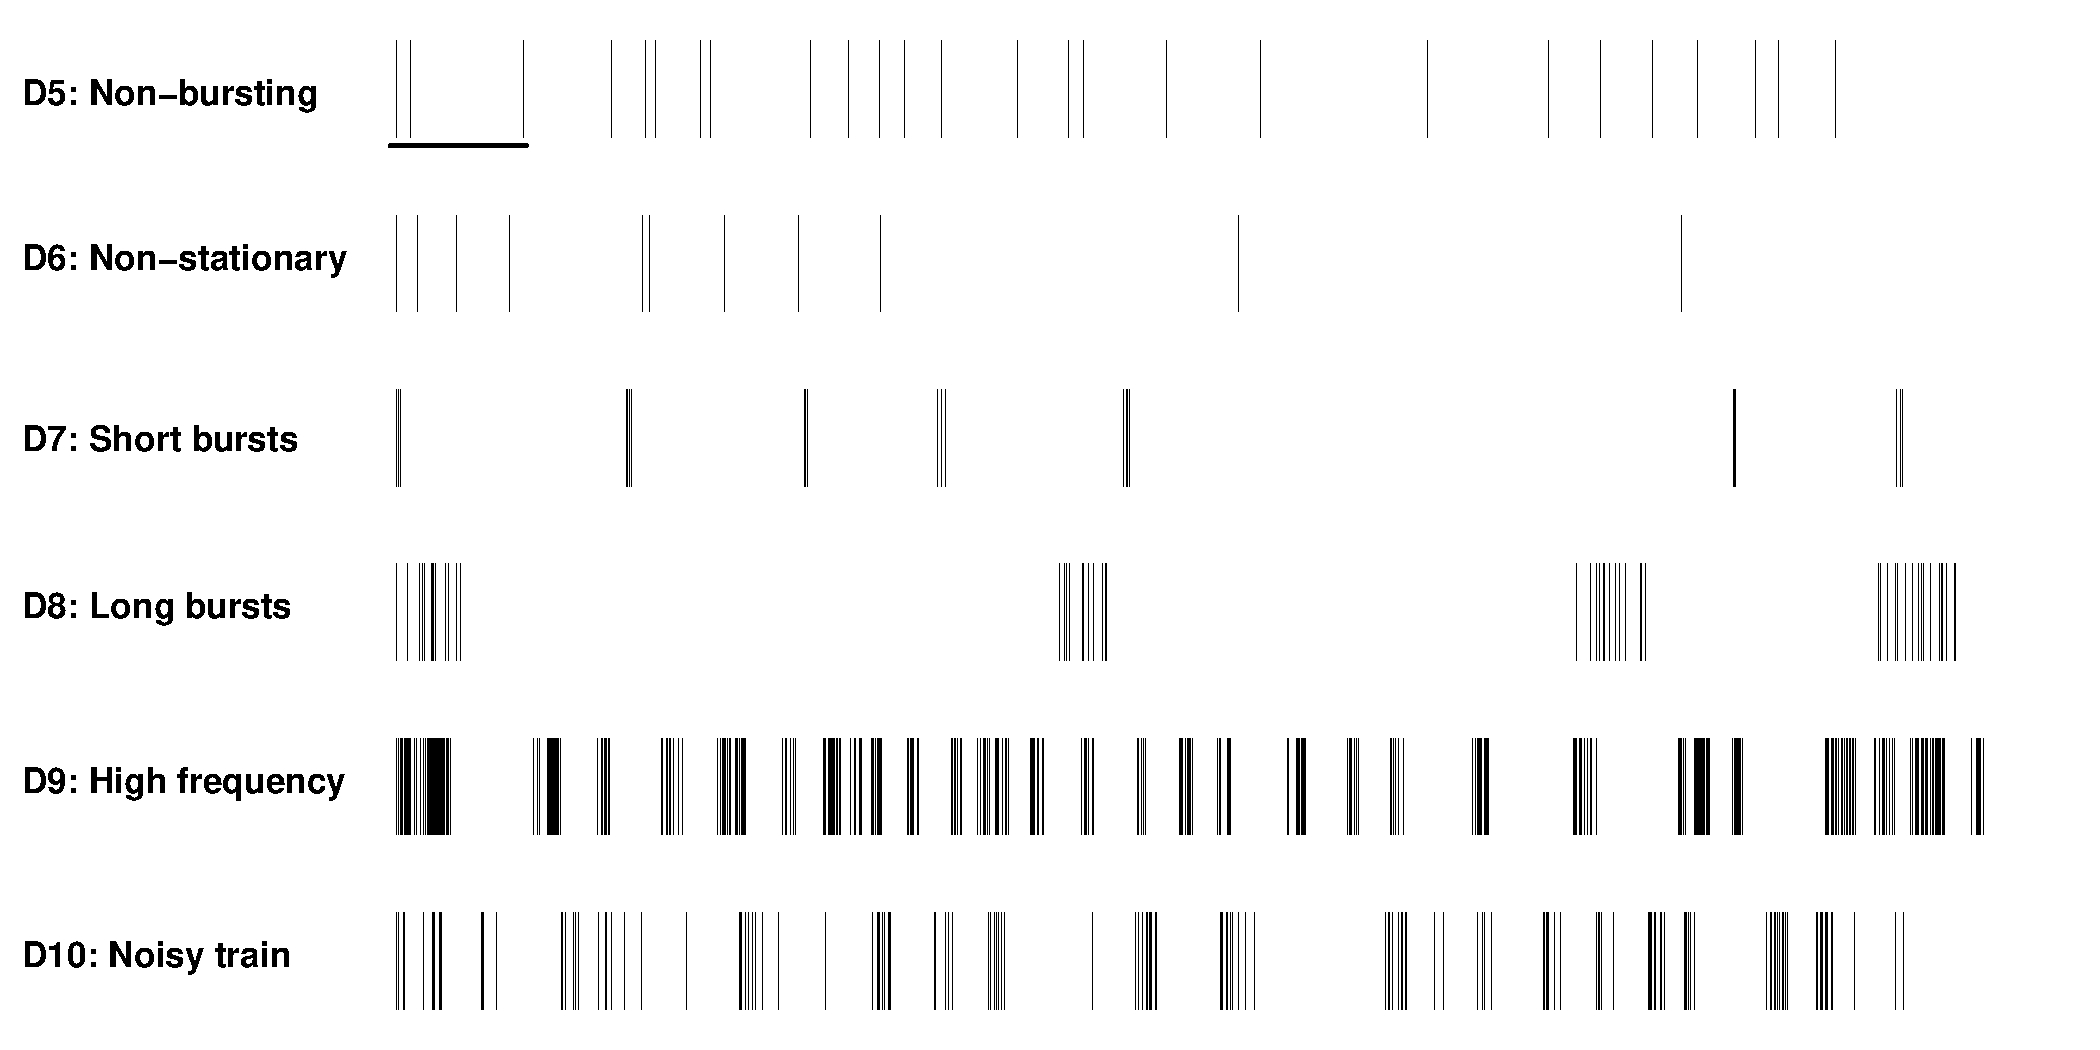
\includegraphics[width=170mm]{sim_egs.pdf}}
			\caption{One minute examples of simulated spike trains for evaluating desirable features D5-D10. Scale bar represents 5$\,$s.}
			\label{sim_egs}
		\end{figure}
		\begin{figure}
			\centering
			\fbox{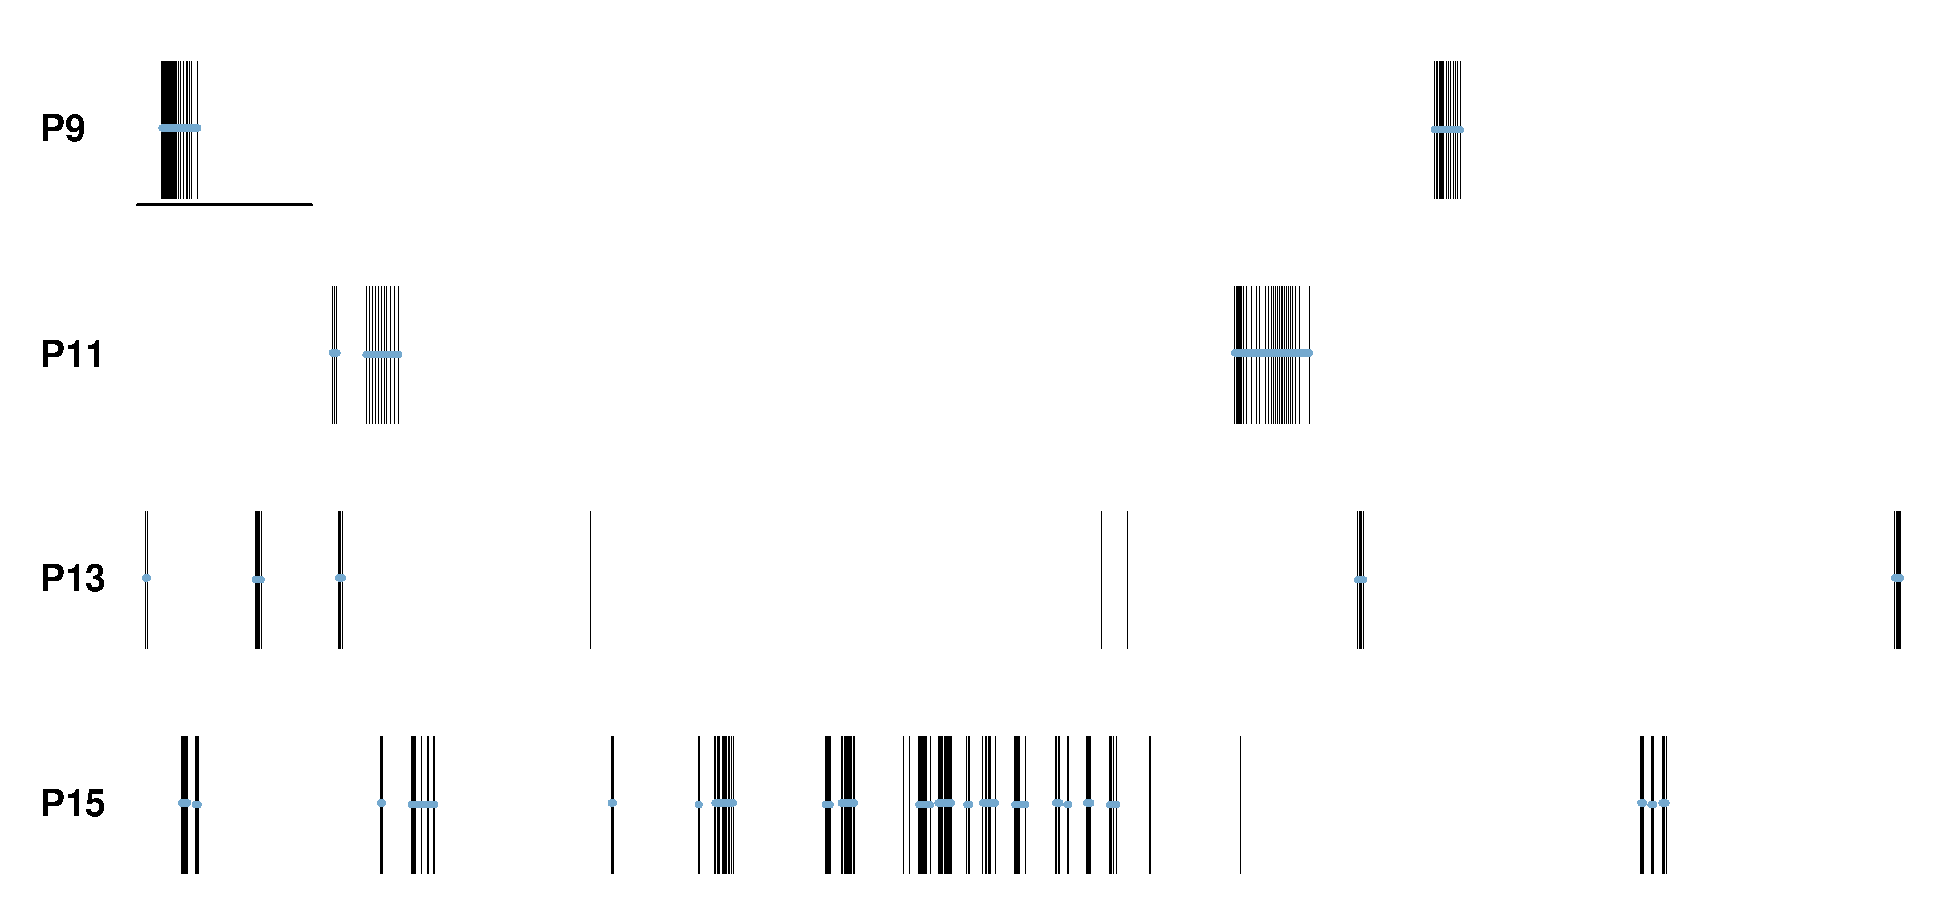
\includegraphics[width=140mm]{rgc_eg_data.pdf}}
			\caption{Examples of one minute spike trains from recordings of mouse retinal ganglion cell at each postnatal day. Horizontal blue bars represent bursts annotated by a human observer. Scale bar represents 5$\,$s of activity. Raw data available from \protect\cite{Eglen2014a}.}
			\label{RGC_eg}
		\end{figure}
		\begin{figure}[h]
			\centering
			\fbox{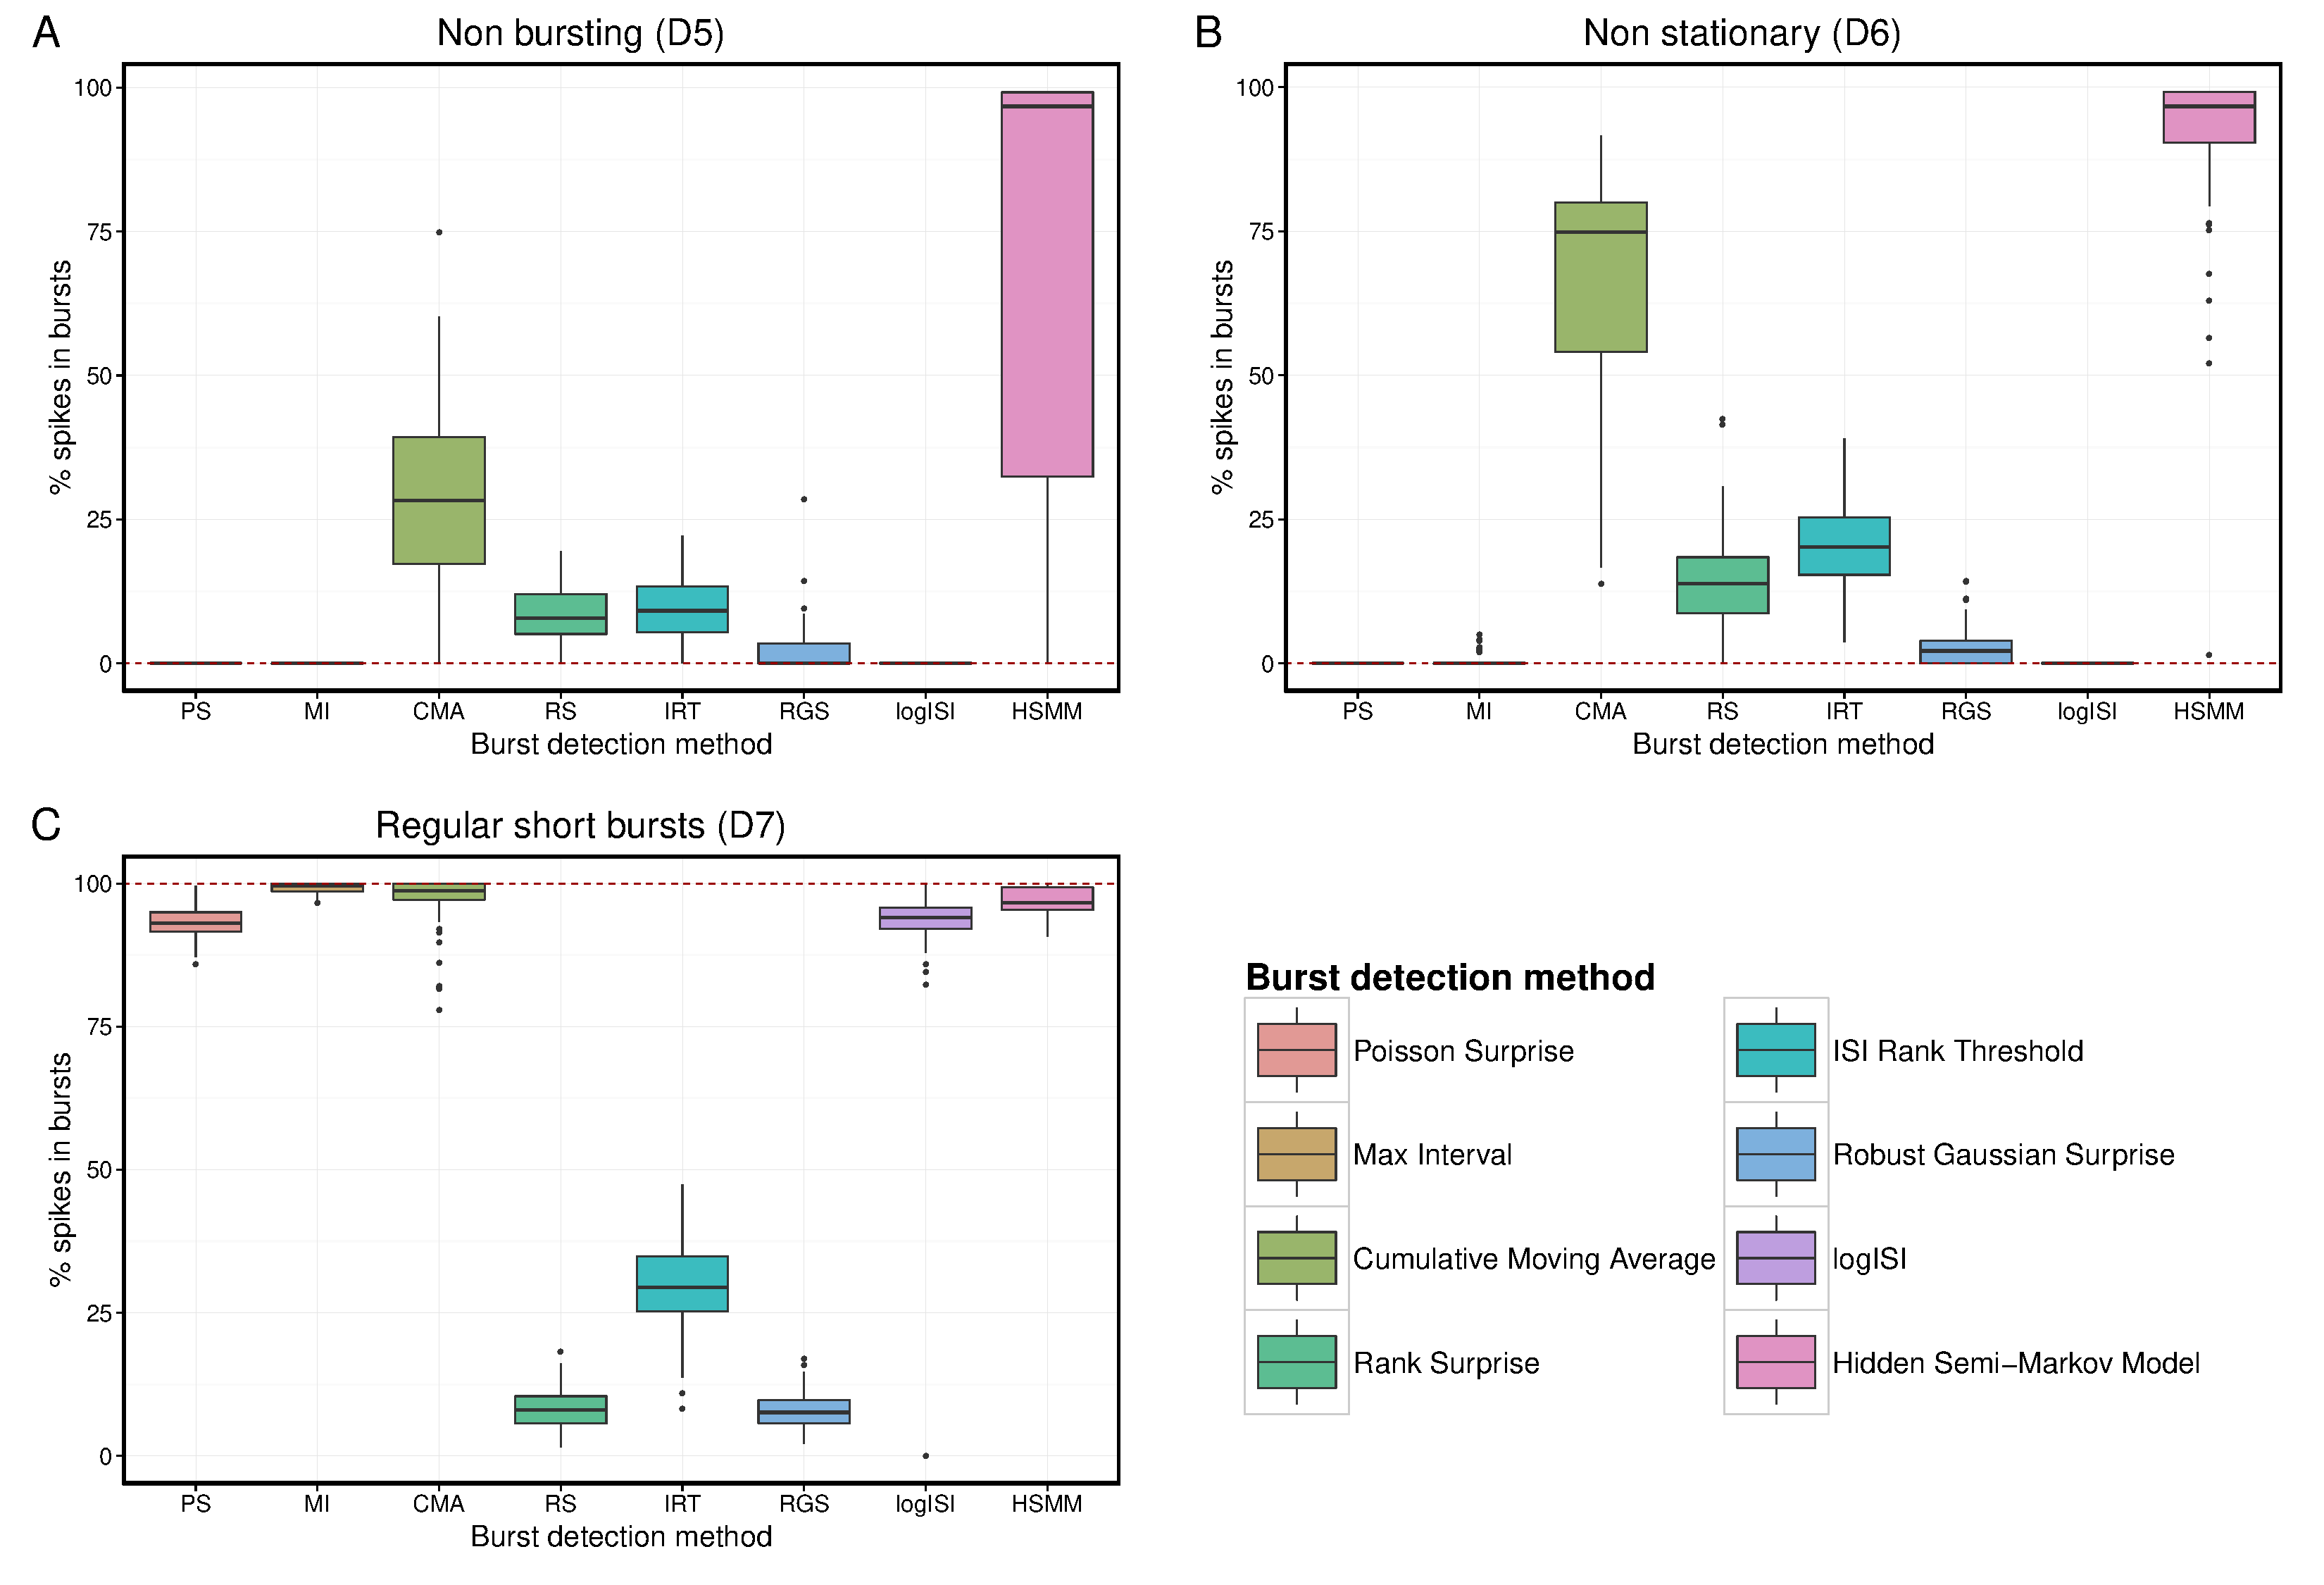
\includegraphics[width=170mm]{des_feat_results1.pdf}}
			\caption{Percentage of spikes in bursts found by each method over 100 simulated trains with \textbf{A} No bursting (D5), \textbf{B}  No bursting and non-stationary firing rate (D6), \textbf{C} Short regular bursts (D7). Dotted line shows desired result from ideal burst detection. Methods close to this line are deemed to work well.}
			\label{sim_results1}
		\end{figure}
		\begin{figure}
			\centering
			\fbox{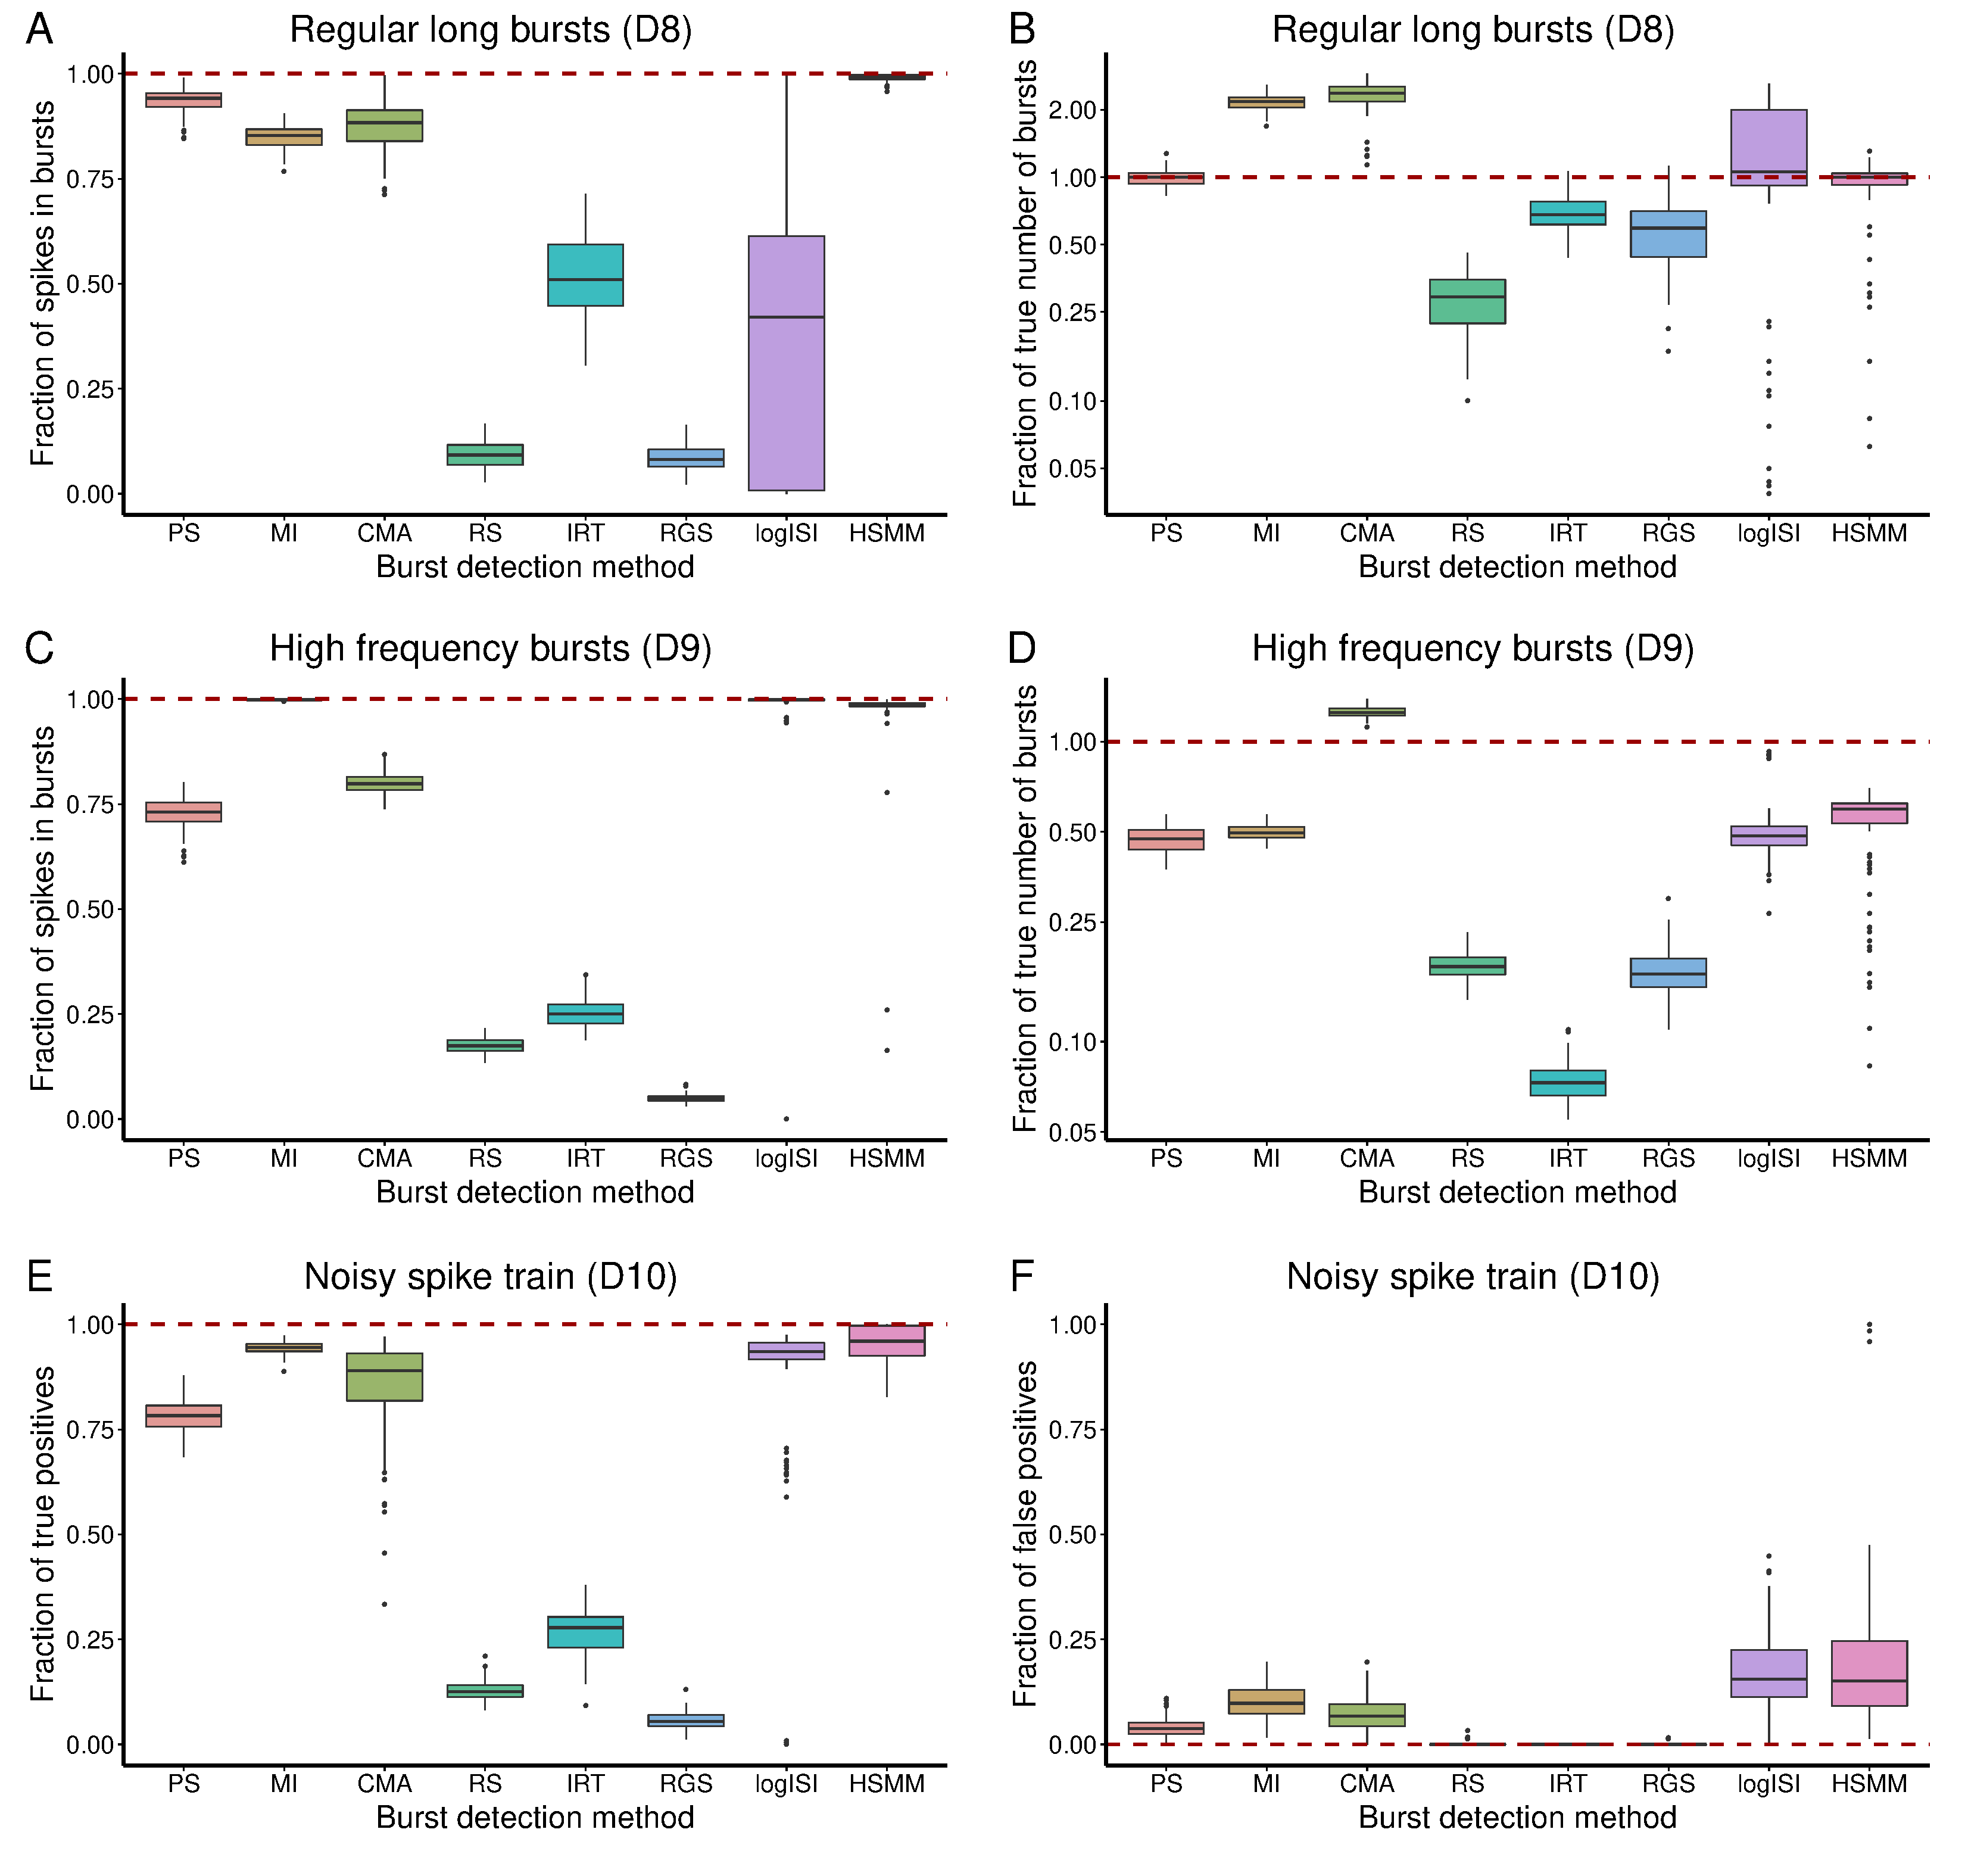
\includegraphics[width=170mm]{des_feat_results2.pdf}}
			\caption{Results of each burst detection method over 100 simulated spike trains. \textbf{A} Percentage of spikes in bursts, and \textbf{B} Number of bursts found by each method relative to the true number of bursts on trains with regular long bursts (D8); \textbf{C} Percentage of spikes in bursts, and \textbf{D} Number of bursts found by each method relative to the true number of bursts on trains with high frequency bursting (D9); \textbf{E} Fraction of true positive, and \textbf{F} Fraction of false positive spikes in bursts found in trains containing both bursting and noise (D10). Dotted line as per Figure \ref{sim_results1} legend. \textbf{B} and \textbf{D} are presented on a log-scale.}
			\label{sim_results2}
		\end{figure}	
		\begin{figure}[h]
			\centering
			%\fbox{\includegraphics[width=170mm]{paper_ROC2.pdf}}
			\fbox{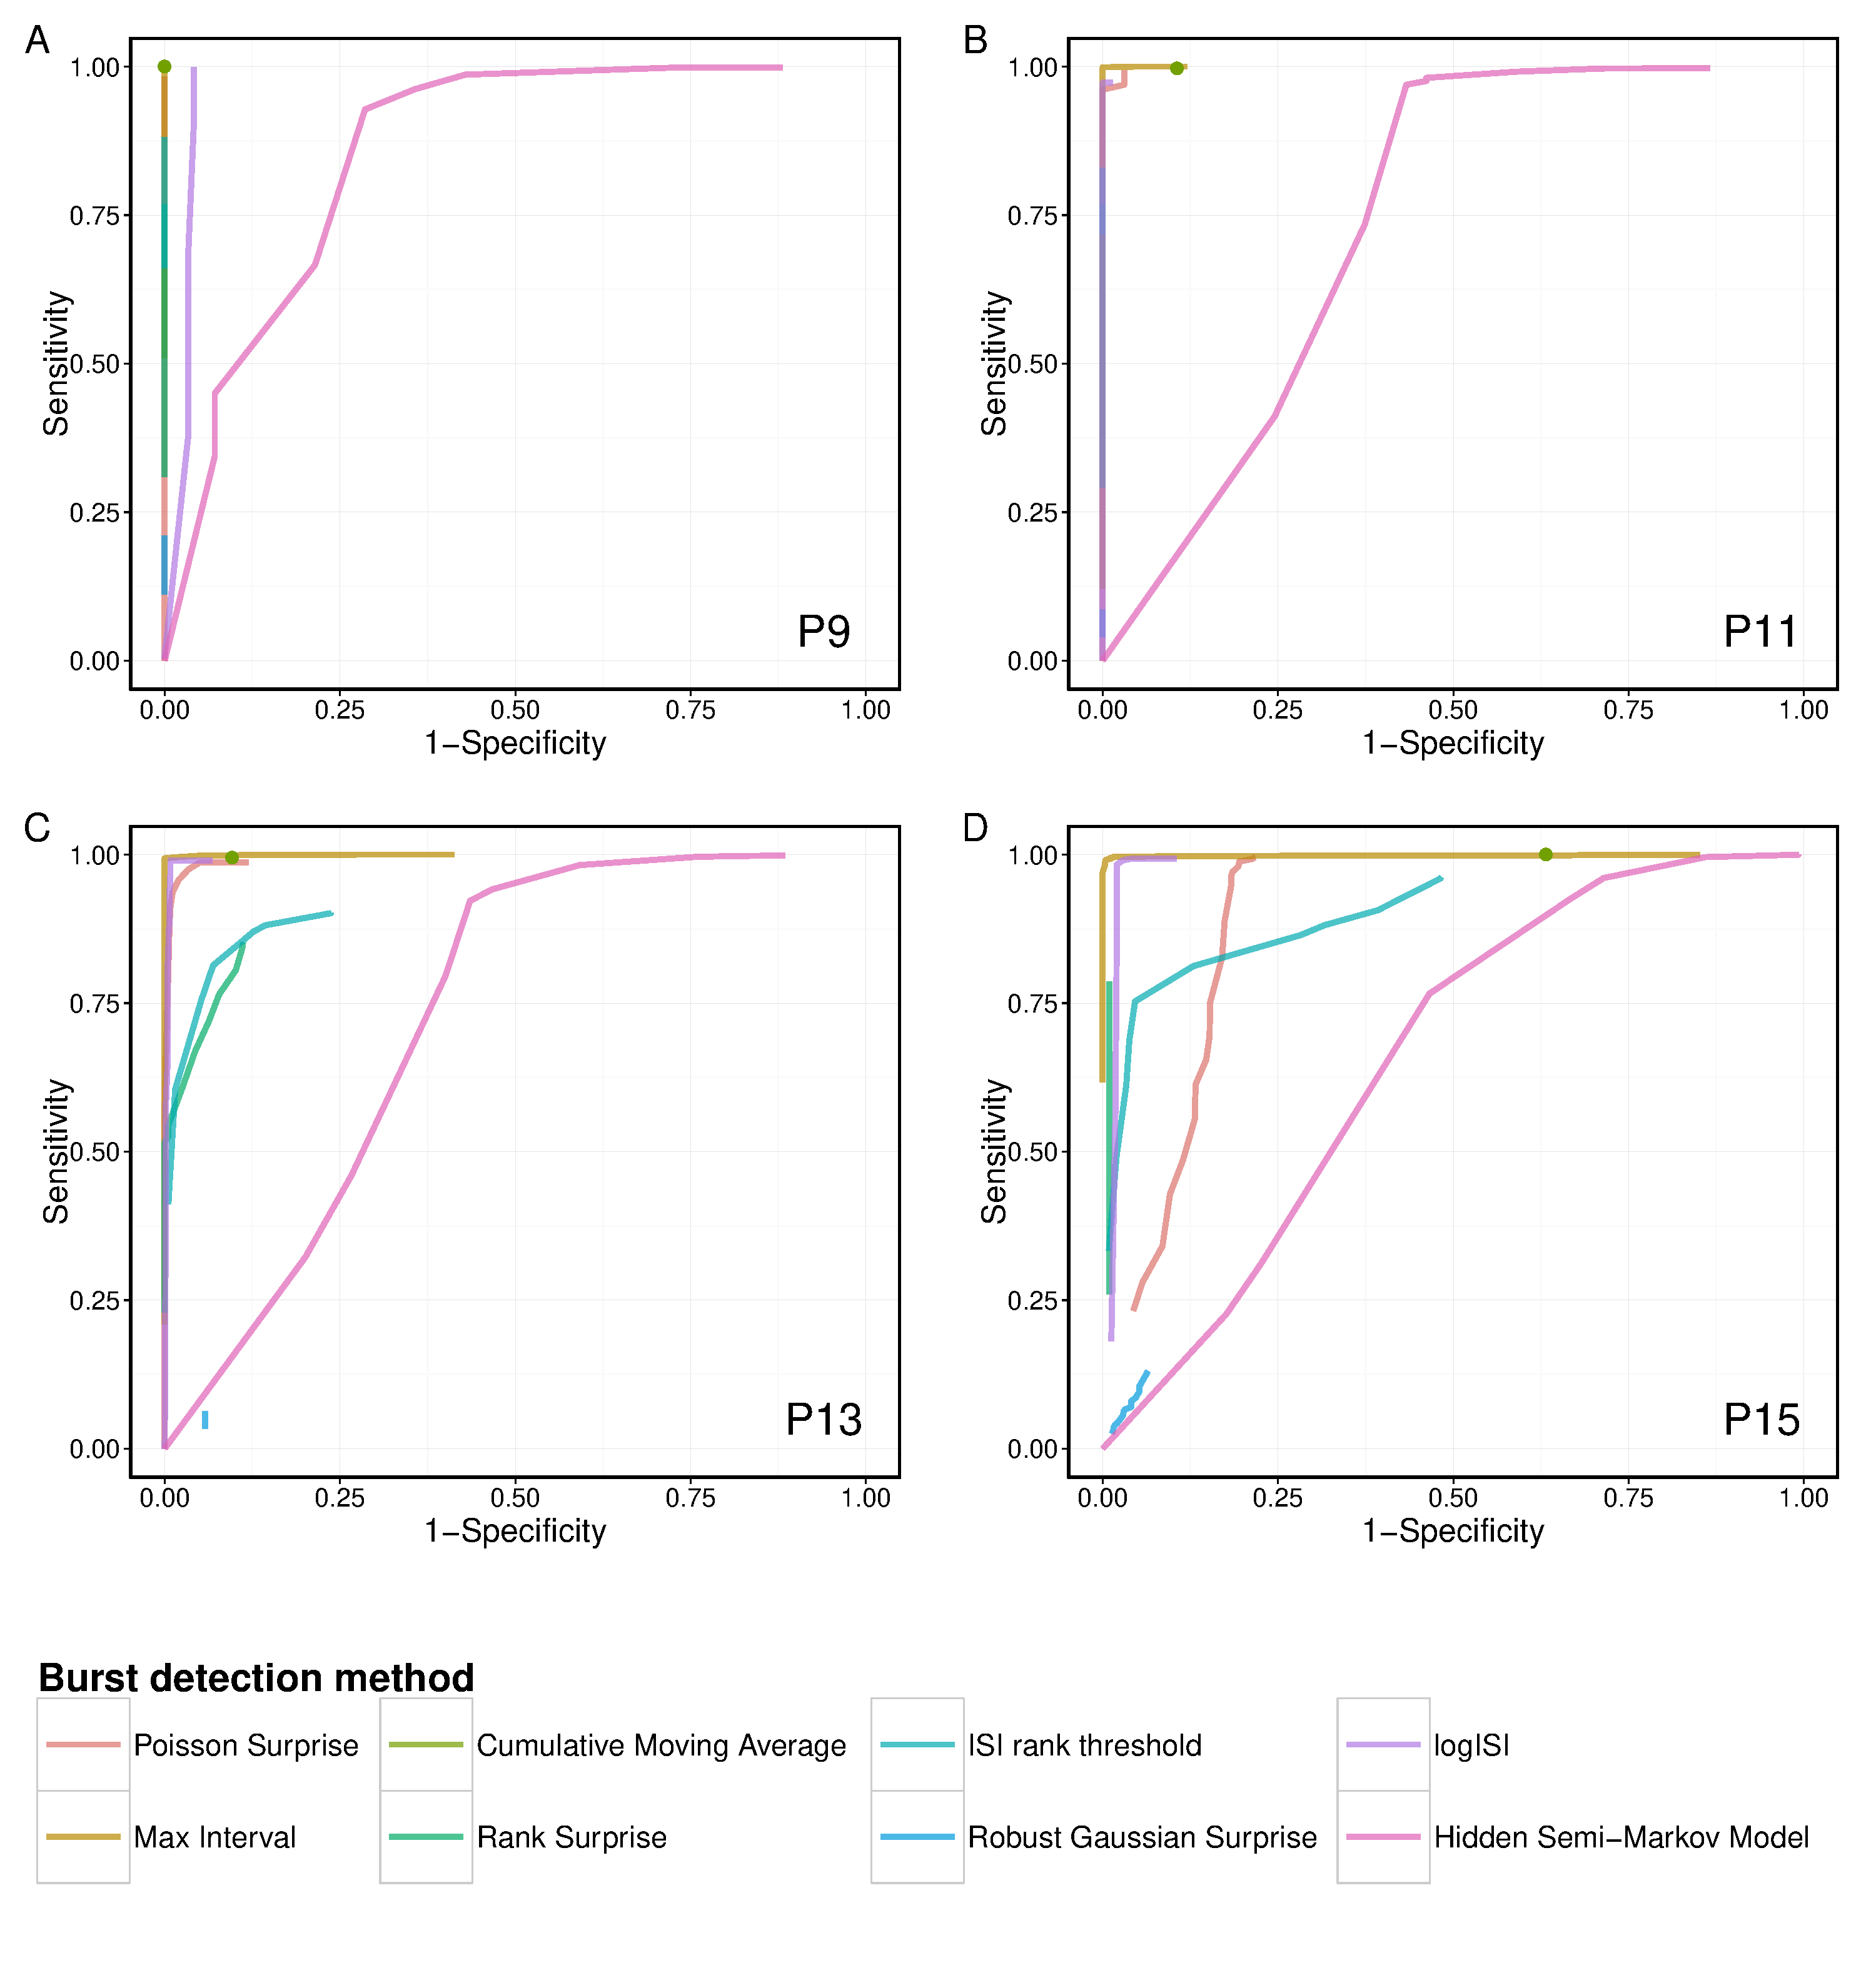
\includegraphics[width=170mm]{RGC_ROC.pdf}}
			\caption{ROC curves showing fraction of true positive and false positive spikes identified as being within bursts for a variety of input parameter values, for recordings of mouse retina, ganglion cells at \textbf{A} P9, \textbf{B} P11,  \textbf{C} P13 and \textbf{D} P15. The ground truth bursts for hour-long recordings of five randomly selected electrodes at each DIV were determined by visual inspection, examples of which are shown in Figure \ref{RGC_eg}, and the mean performance of each method over the five electrodes is shown.}
			\label{ROC}
		\end{figure}  
		\begin{figure}[h]
			\centering
			\fbox{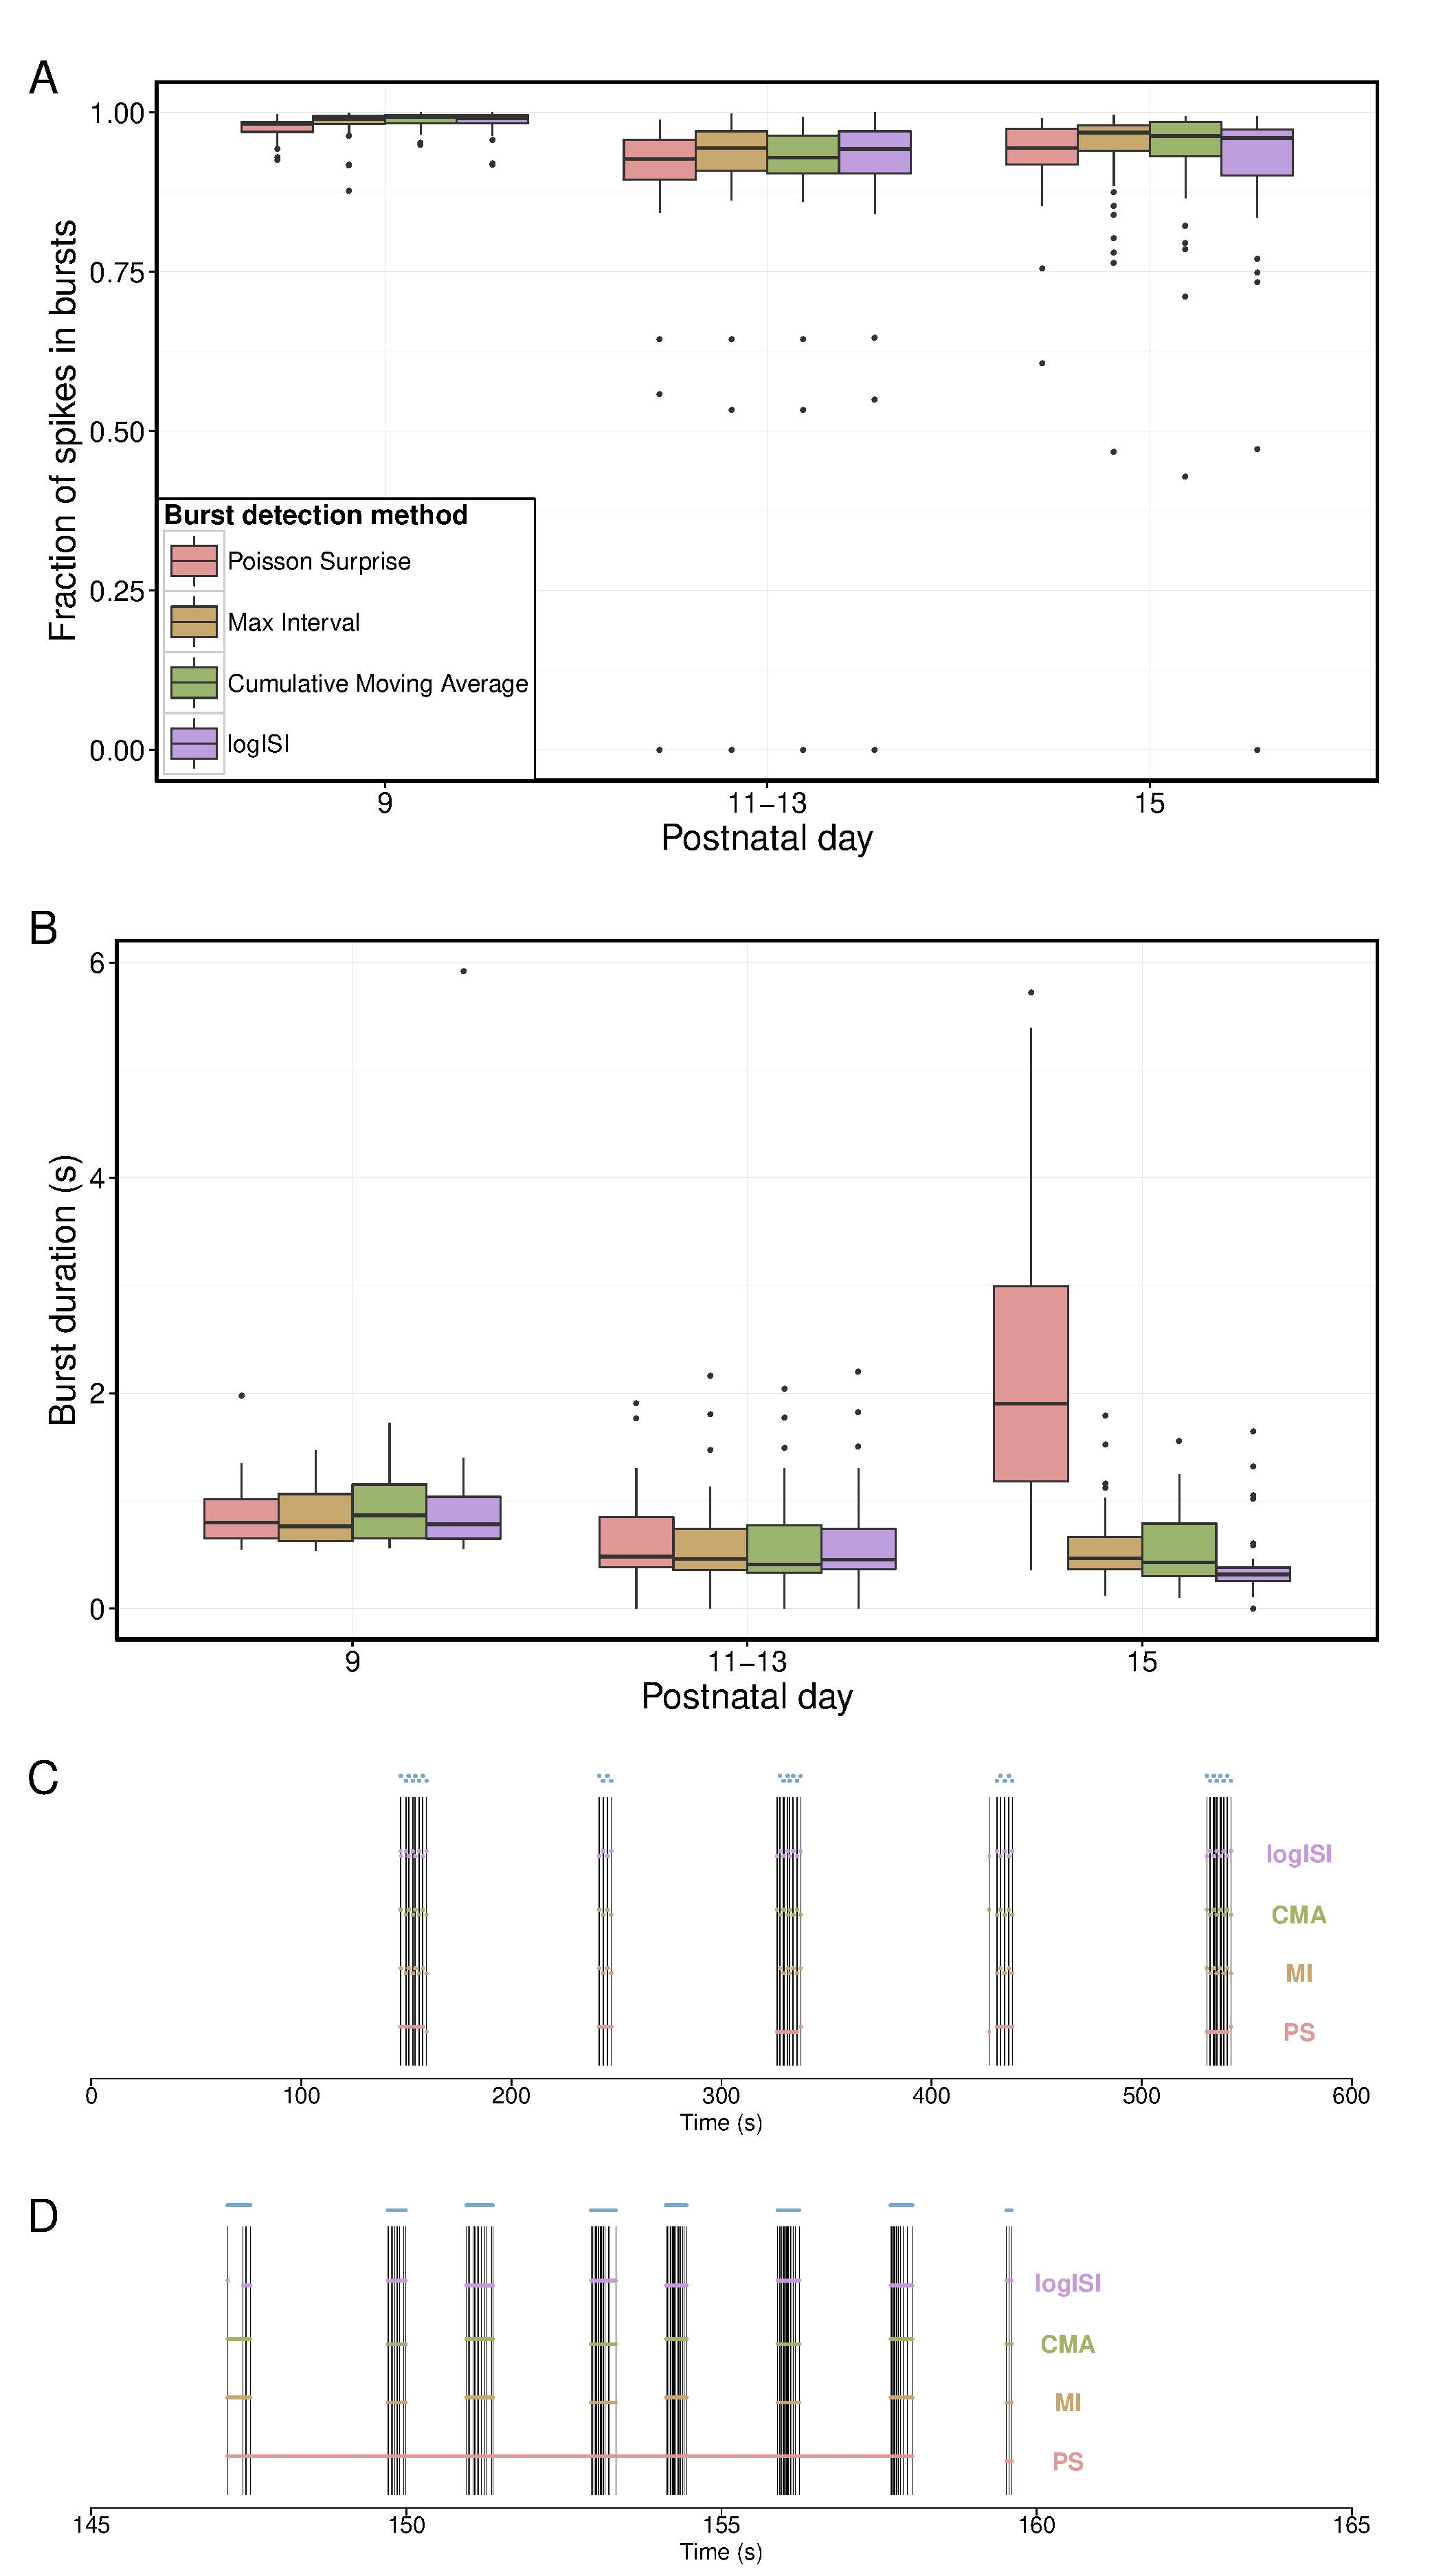
\includegraphics[width=120mm]{RGC_analysis.pdf}}
			\caption{Detailed analysis of mouse RGC data. \textbf{A} Percentage of spikes in bursts, \textbf{B} Mean burst duration, \textbf{C} Bursts detected by each method over 1000$\,$s sample of a P15 spike train, and \textbf{D} 20$\,$s sample showing the first burst from the same spike train. Each electrode was counted as one data point in the box plots. The legend in \textbf{A} applies to both \textbf{A} and \textbf{B}.}
			\label{RGC_results}
		\end{figure}
		\begin{table}[h]
			\centering
			\begin{tabular}{|l|l|l|}
				\hline
				Method & Parameter & Value
				\\ \hline 
				\rowcolor{Gray} LogISI & Maximum cutoff value & 150$\,$ms
				\\ \hline
				CMA & $\alpha_1 (\alpha_2)$ & 1 (0.5) if skew $<1$
				\\ & &  0.7 (0.5) if $1 \leq $ skew $<4$
				\\ & & 0.5 (0.9) if $4 \leq $ skew $<9$
				\\ & & 0.3 (0.1) if  skew $\geq 9$
				\\ & Maximum mean burst duration & 5$\,$s
				\\ & Maximum mean spikes per burst & 50
				\\ \hline 
				\rowcolor{Gray} Poisson Surprise  & Minimum surprise value & $-\log(0.0025) \approx 6$\\ \hline 
				MaxInterval & Maximum beginning ISI & 0.2$\,$s
				\\ & Maximum end ISI & 0.25$\,$s
				\\ & Minimum inter-burst interval & 0.2$\,$s
				\\ & Minimum burst duration & 0.01$\,$s
				\\ & Minimum spikes in a burst & 3
				\\ \hline
			\end{tabular}
			\caption{Parameter values used for burst detection on hiPSC-derived neuronal networks}
			\label{param_vals_hum}
		\end{table}
		\begin{figure}[h]
			\centering
			\fbox{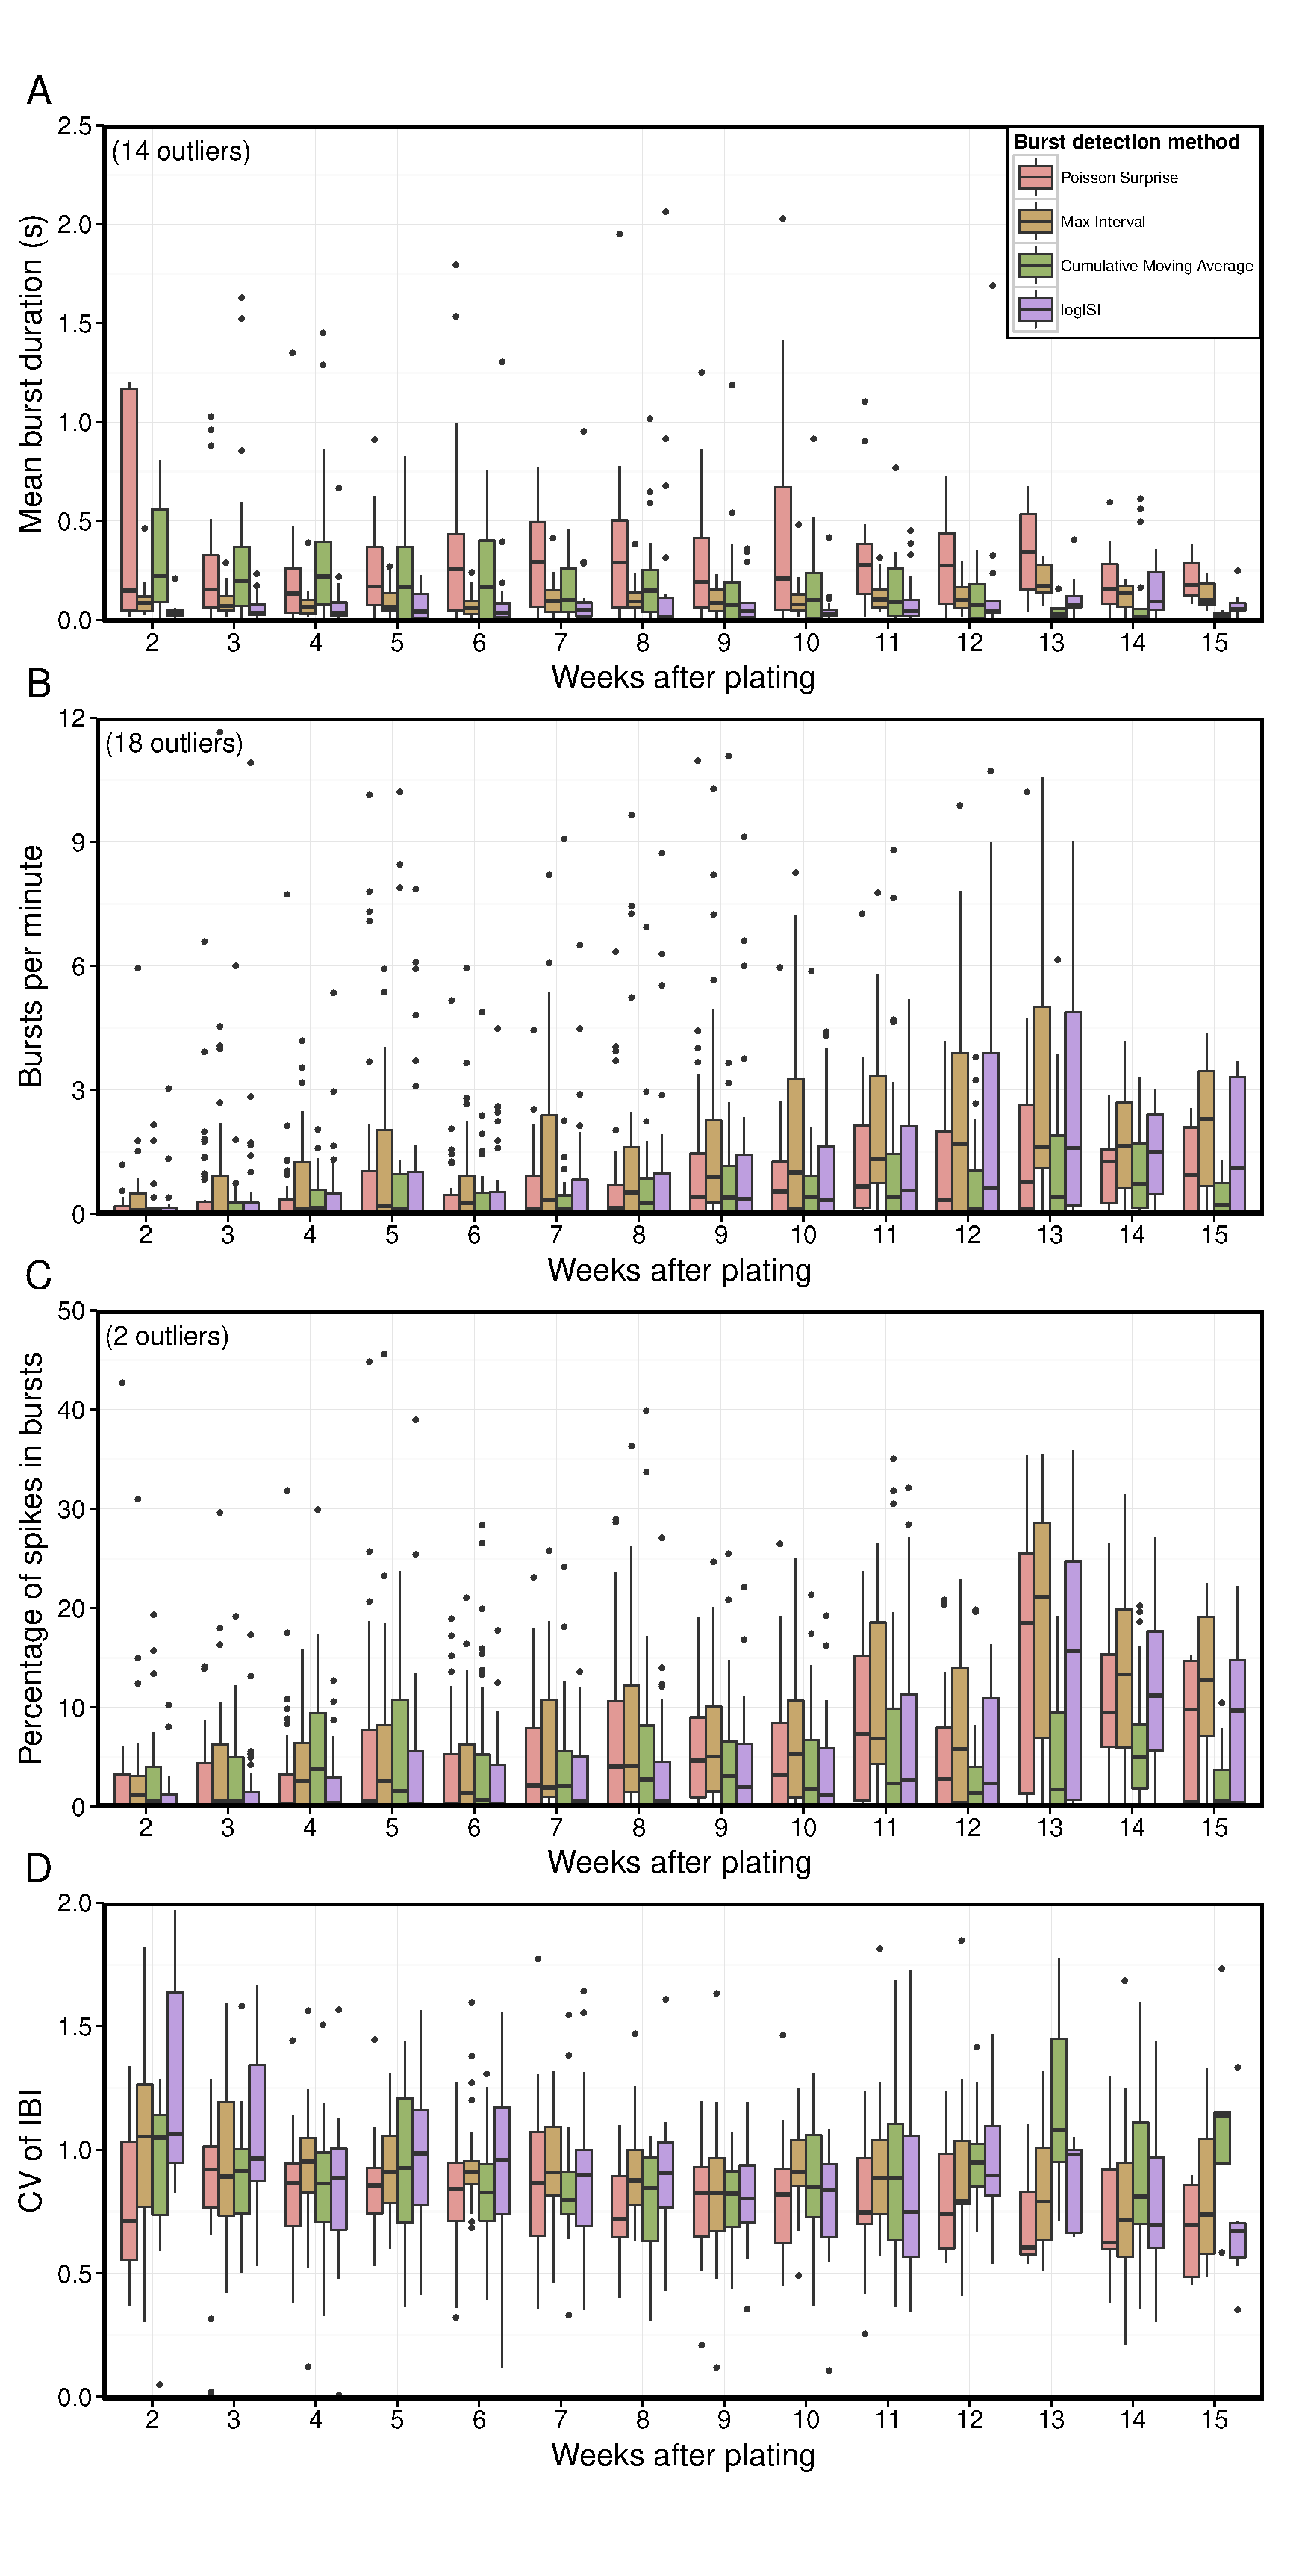
\includegraphics[width=115mm]{hiPSN_analysis.pdf}}
			\caption{Analysis of recordings of networks of hiPSC-derived neurons. \textbf{A} Mean burst duration, \textbf{B} Bursts per minute, \textbf{C} Percentage of spikes in bursts, and \textbf{D} CV of IBI}
			\label{hiPSN_results}
		\end{figure}
		\begin{figure}[h]
			\centering
			\fbox{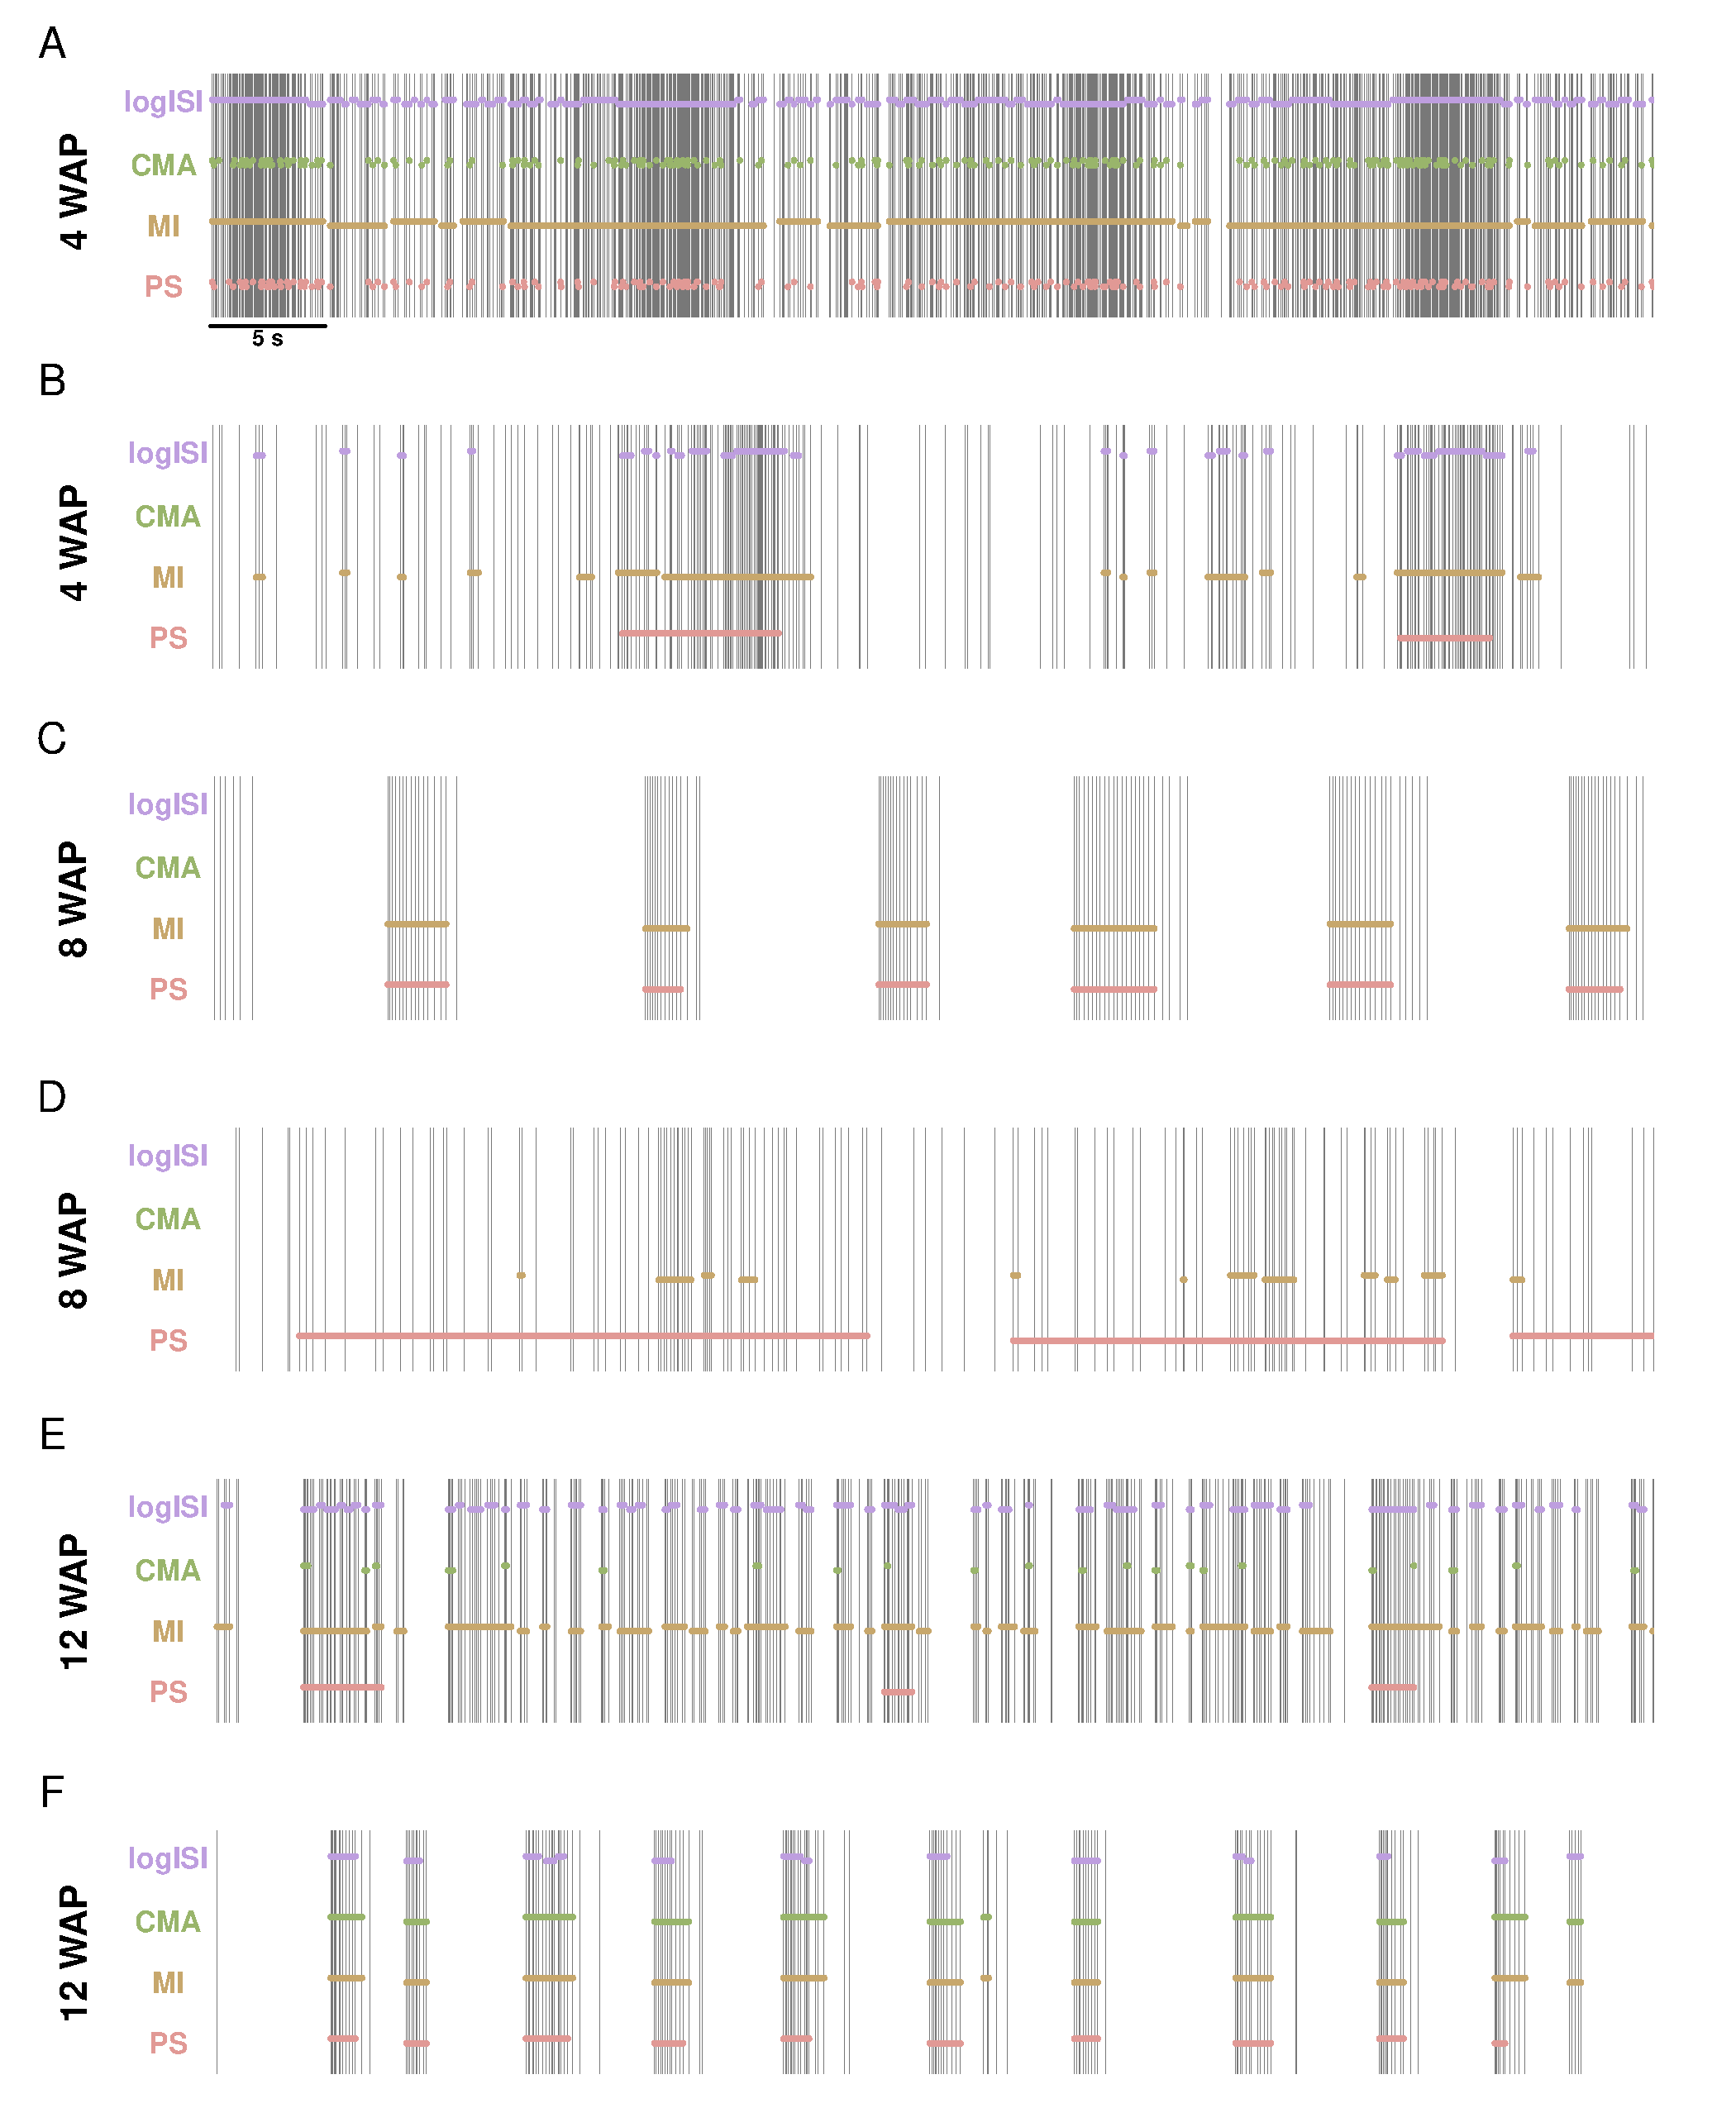
\includegraphics[width=140mm]{hiPSN_egs.pdf}}
			\caption{Burst detection results of the four analysis methods on 60$\,$s samples of human neuronal network recordings at \textbf{A, B} 4 weeks after plating (WAP), \textbf{C, D} 8 WAP, and \textbf{E, F} 12 WAP. Scale bar represents 5$\,$s.}
			\label{hiPSN_examples}
		\end{figure}
		\clearpage
		\bibliographystyle{jneurosci} 
		\bibliography{Bursting.bib}
	\end{document}